% Options for packages loaded elsewhere
\PassOptionsToPackage{unicode}{hyperref}
\PassOptionsToPackage{hyphens}{url}
%
\documentclass[
]{article}
\usepackage{amsmath,amssymb}
\usepackage{lmodern}
\usepackage{iftex}
\ifPDFTeX
  \usepackage[T1]{fontenc}
  \usepackage[utf8]{inputenc}
  \usepackage{textcomp} % provide euro and other symbols
\else % if luatex or xetex
  \usepackage{unicode-math}
  \defaultfontfeatures{Scale=MatchLowercase}
  \defaultfontfeatures[\rmfamily]{Ligatures=TeX,Scale=1}
\fi
% Use upquote if available, for straight quotes in verbatim environments
\IfFileExists{upquote.sty}{\usepackage{upquote}}{}
\IfFileExists{microtype.sty}{% use microtype if available
  \usepackage[]{microtype}
  \UseMicrotypeSet[protrusion]{basicmath} % disable protrusion for tt fonts
}{}
\makeatletter
\@ifundefined{KOMAClassName}{% if non-KOMA class
  \IfFileExists{parskip.sty}{%
    \usepackage{parskip}
  }{% else
    \setlength{\parindent}{0pt}
    \setlength{\parskip}{6pt plus 2pt minus 1pt}}
}{% if KOMA class
  \KOMAoptions{parskip=half}}
\makeatother
\usepackage{xcolor}
\usepackage[margin=1in]{geometry}
\usepackage{color}
\usepackage{fancyvrb}
\newcommand{\VerbBar}{|}
\newcommand{\VERB}{\Verb[commandchars=\\\{\}]}
\DefineVerbatimEnvironment{Highlighting}{Verbatim}{commandchars=\\\{\}}
% Add ',fontsize=\small' for more characters per line
\usepackage{framed}
\definecolor{shadecolor}{RGB}{248,248,248}
\newenvironment{Shaded}{\begin{snugshade}}{\end{snugshade}}
\newcommand{\AlertTok}[1]{\textcolor[rgb]{0.94,0.16,0.16}{#1}}
\newcommand{\AnnotationTok}[1]{\textcolor[rgb]{0.56,0.35,0.01}{\textbf{\textit{#1}}}}
\newcommand{\AttributeTok}[1]{\textcolor[rgb]{0.77,0.63,0.00}{#1}}
\newcommand{\BaseNTok}[1]{\textcolor[rgb]{0.00,0.00,0.81}{#1}}
\newcommand{\BuiltInTok}[1]{#1}
\newcommand{\CharTok}[1]{\textcolor[rgb]{0.31,0.60,0.02}{#1}}
\newcommand{\CommentTok}[1]{\textcolor[rgb]{0.56,0.35,0.01}{\textit{#1}}}
\newcommand{\CommentVarTok}[1]{\textcolor[rgb]{0.56,0.35,0.01}{\textbf{\textit{#1}}}}
\newcommand{\ConstantTok}[1]{\textcolor[rgb]{0.00,0.00,0.00}{#1}}
\newcommand{\ControlFlowTok}[1]{\textcolor[rgb]{0.13,0.29,0.53}{\textbf{#1}}}
\newcommand{\DataTypeTok}[1]{\textcolor[rgb]{0.13,0.29,0.53}{#1}}
\newcommand{\DecValTok}[1]{\textcolor[rgb]{0.00,0.00,0.81}{#1}}
\newcommand{\DocumentationTok}[1]{\textcolor[rgb]{0.56,0.35,0.01}{\textbf{\textit{#1}}}}
\newcommand{\ErrorTok}[1]{\textcolor[rgb]{0.64,0.00,0.00}{\textbf{#1}}}
\newcommand{\ExtensionTok}[1]{#1}
\newcommand{\FloatTok}[1]{\textcolor[rgb]{0.00,0.00,0.81}{#1}}
\newcommand{\FunctionTok}[1]{\textcolor[rgb]{0.00,0.00,0.00}{#1}}
\newcommand{\ImportTok}[1]{#1}
\newcommand{\InformationTok}[1]{\textcolor[rgb]{0.56,0.35,0.01}{\textbf{\textit{#1}}}}
\newcommand{\KeywordTok}[1]{\textcolor[rgb]{0.13,0.29,0.53}{\textbf{#1}}}
\newcommand{\NormalTok}[1]{#1}
\newcommand{\OperatorTok}[1]{\textcolor[rgb]{0.81,0.36,0.00}{\textbf{#1}}}
\newcommand{\OtherTok}[1]{\textcolor[rgb]{0.56,0.35,0.01}{#1}}
\newcommand{\PreprocessorTok}[1]{\textcolor[rgb]{0.56,0.35,0.01}{\textit{#1}}}
\newcommand{\RegionMarkerTok}[1]{#1}
\newcommand{\SpecialCharTok}[1]{\textcolor[rgb]{0.00,0.00,0.00}{#1}}
\newcommand{\SpecialStringTok}[1]{\textcolor[rgb]{0.31,0.60,0.02}{#1}}
\newcommand{\StringTok}[1]{\textcolor[rgb]{0.31,0.60,0.02}{#1}}
\newcommand{\VariableTok}[1]{\textcolor[rgb]{0.00,0.00,0.00}{#1}}
\newcommand{\VerbatimStringTok}[1]{\textcolor[rgb]{0.31,0.60,0.02}{#1}}
\newcommand{\WarningTok}[1]{\textcolor[rgb]{0.56,0.35,0.01}{\textbf{\textit{#1}}}}
\usepackage{graphicx}
\makeatletter
\def\maxwidth{\ifdim\Gin@nat@width>\linewidth\linewidth\else\Gin@nat@width\fi}
\def\maxheight{\ifdim\Gin@nat@height>\textheight\textheight\else\Gin@nat@height\fi}
\makeatother
% Scale images if necessary, so that they will not overflow the page
% margins by default, and it is still possible to overwrite the defaults
% using explicit options in \includegraphics[width, height, ...]{}
\setkeys{Gin}{width=\maxwidth,height=\maxheight,keepaspectratio}
% Set default figure placement to htbp
\makeatletter
\def\fps@figure{htbp}
\makeatother
\setlength{\emergencystretch}{3em} % prevent overfull lines
\providecommand{\tightlist}{%
  \setlength{\itemsep}{0pt}\setlength{\parskip}{0pt}}
\setcounter{secnumdepth}{-\maxdimen} % remove section numbering
\ifLuaTeX
  \usepackage{selnolig}  % disable illegal ligatures
\fi
\IfFileExists{bookmark.sty}{\usepackage{bookmark}}{\usepackage{hyperref}}
\IfFileExists{xurl.sty}{\usepackage{xurl}}{} % add URL line breaks if available
\urlstyle{same} % disable monospaced font for URLs
\hypersetup{
  pdftitle={Arrival At Carcasses},
  pdfauthor={Kaija Gahm},
  hidelinks,
  pdfcreator={LaTeX via pandoc}}

\title{Arrival At Carcasses}
\author{Kaija Gahm}
\date{2022-10-10}

\begin{document}
\maketitle

\begin{Shaded}
\begin{Highlighting}[]
\FunctionTok{library}\NormalTok{(tidyverse)}
\end{Highlighting}
\end{Shaded}

\begin{verbatim}
## -- Attaching packages --------------------------------------- tidyverse 1.3.2 --
## v ggplot2 3.3.6      v purrr   0.3.5 
## v tibble  3.1.8      v dplyr   1.0.10
## v tidyr   1.2.1      v stringr 1.4.1 
## v readr   2.1.3      v forcats 0.5.2 
## -- Conflicts ------------------------------------------ tidyverse_conflicts() --
## x dplyr::filter() masks stats::filter()
## x dplyr::lag()    masks stats::lag()
\end{verbatim}

\begin{Shaded}
\begin{Highlighting}[]
\FunctionTok{library}\NormalTok{(vultureUtils)}
\FunctionTok{library}\NormalTok{(igraph)}
\end{Highlighting}
\end{Shaded}

\begin{verbatim}
## 
## Attaching package: 'igraph'
## 
## The following objects are masked from 'package:dplyr':
## 
##     as_data_frame, groups, union
## 
## The following objects are masked from 'package:purrr':
## 
##     compose, simplify
## 
## The following object is masked from 'package:tidyr':
## 
##     crossing
## 
## The following object is masked from 'package:tibble':
## 
##     as_data_frame
## 
## The following objects are masked from 'package:stats':
## 
##     decompose, spectrum
## 
## The following object is masked from 'package:base':
## 
##     union
\end{verbatim}

\begin{Shaded}
\begin{Highlighting}[]
\FunctionTok{library}\NormalTok{(elevatr) }\CommentTok{\# for getting elevation data}
\FunctionTok{library}\NormalTok{(suncalc) }\CommentTok{\# for calculating sunrise and sunset}
\FunctionTok{library}\NormalTok{(ggmap)}
\end{Highlighting}
\end{Shaded}

\begin{verbatim}
## Google's Terms of Service: https://cloud.google.com/maps-platform/terms/.
## Please cite ggmap if you use it! See citation("ggmap") for details.
\end{verbatim}

\begin{Shaded}
\begin{Highlighting}[]
\FunctionTok{source}\NormalTok{(}\StringTok{"bboxFromRad.R"}\NormalTok{)}
\FunctionTok{library}\NormalTok{(units)}
\end{Highlighting}
\end{Shaded}

\begin{verbatim}
## udunits database from /Users/kaijagahmpersonalprojects/Library/Application Support/renv/cache/v5/R-4.2/x86_64-apple-darwin17.0/units/0.8-0/6c374b265ba437f8d384ec7a313edd96/units/share/udunits/udunits2.xml
\end{verbatim}

\begin{Shaded}
\begin{Highlighting}[]
\FunctionTok{library}\NormalTok{(tidyverse)}
\FunctionTok{library}\NormalTok{(sf)}
\end{Highlighting}
\end{Shaded}

\begin{verbatim}
## Linking to GEOS 3.10.2, GDAL 3.4.2, PROJ 8.2.1; sf_use_s2() is TRUE
\end{verbatim}

\begin{Shaded}
\begin{Highlighting}[]
\FunctionTok{library}\NormalTok{(gganimate)}
\FunctionTok{library}\NormalTok{(rnaturalearth)}
\FunctionTok{library}\NormalTok{(gifski)}
\end{Highlighting}
\end{Shaded}

\begin{Shaded}
\begin{Highlighting}[]
\NormalTok{datAnnot }\OtherTok{\textless{}{-}}\NormalTok{ feather}\SpecialCharTok{::}\FunctionTok{read\_feather}\NormalTok{(}\StringTok{"data/datAnnot.feather"}\NormalTok{)}
\end{Highlighting}
\end{Shaded}

\hypertarget{analyzing-arrival-order-at-carcasses}{%
\section{Analyzing arrival order at
carcasses}\label{analyzing-arrival-order-at-carcasses}}

\hypertarget{identify-feeding-events}{%
\subsection{IDENTIFY FEEDING EVENTS}\label{identify-feeding-events}}

Let's move on to examining an individual's movement patterns to identify
arrival at a carcass site. Going to pick the individual with the longest
run:

\begin{Shaded}
\begin{Highlighting}[]
\NormalTok{targetIndiv }\OtherTok{\textless{}{-}}\NormalTok{ datAnnot }\SpecialCharTok{\%\textgreater{}\%}
\NormalTok{  dplyr}\SpecialCharTok{::}\FunctionTok{select}\NormalTok{(trackId, longestRun) }\SpecialCharTok{\%\textgreater{}\%}
  \FunctionTok{distinct}\NormalTok{() }\SpecialCharTok{\%\textgreater{}\%}
  \FunctionTok{arrange}\NormalTok{(}\SpecialCharTok{{-}}\NormalTok{longestRun) }\SpecialCharTok{\%\textgreater{}\%}
  \FunctionTok{slice}\NormalTok{(}\DecValTok{1}\NormalTok{) }\SpecialCharTok{\%\textgreater{}\%}
  \FunctionTok{pull}\NormalTok{(trackId)}

\NormalTok{track }\OtherTok{\textless{}{-}}\NormalTok{ datAnnot }\SpecialCharTok{\%\textgreater{}\%}
  \FunctionTok{filter}\NormalTok{(trackId }\SpecialCharTok{==}\NormalTok{ targetIndiv)}

\NormalTok{trackDays }\OtherTok{\textless{}{-}}\NormalTok{ track }\SpecialCharTok{\%\textgreater{}\%}
  \FunctionTok{group\_by}\NormalTok{(dateOnly) }\SpecialCharTok{\%\textgreater{}\%}
  \FunctionTok{group\_split}\NormalTok{(}\AttributeTok{.keep =} \ConstantTok{TRUE}\NormalTok{)}
\end{Highlighting}
\end{Shaded}

\hypertarget{acceleration}{%
\subsubsection{Acceleration}\label{acceleration}}

Visualize acceleration

\begin{Shaded}
\begin{Highlighting}[]
\NormalTok{acc }\OtherTok{\textless{}{-}}\NormalTok{ track }\SpecialCharTok{\%\textgreater{}\%}
\NormalTok{  dplyr}\SpecialCharTok{::}\FunctionTok{select}\NormalTok{(dateOnly, timestamp, }\FunctionTok{contains}\NormalTok{(}\StringTok{"acceleration\_"}\NormalTok{)) }\SpecialCharTok{\%\textgreater{}\%}
  \FunctionTok{pivot\_longer}\NormalTok{(}\AttributeTok{cols =} \FunctionTok{contains}\NormalTok{(}\StringTok{"acceleration\_"}\NormalTok{), }\AttributeTok{names\_to =} \StringTok{"axis"}\NormalTok{, }\AttributeTok{values\_to =} \StringTok{"acceleration"}\NormalTok{) }\SpecialCharTok{\%\textgreater{}\%}
  \FunctionTok{mutate}\NormalTok{(}\AttributeTok{axis =} \FunctionTok{str\_remove}\NormalTok{(axis, }\StringTok{"acceleration\_raw\_"}\NormalTok{))}

\NormalTok{acc }\SpecialCharTok{\%\textgreater{}\%}
  \FunctionTok{ggplot}\NormalTok{(}\FunctionTok{aes}\NormalTok{(}\AttributeTok{x =}\NormalTok{ timestamp, }\AttributeTok{y =}\NormalTok{ acceleration, }\AttributeTok{col =}\NormalTok{ axis))}\SpecialCharTok{+}
  \FunctionTok{geom\_line}\NormalTok{()}
\end{Highlighting}
\end{Shaded}

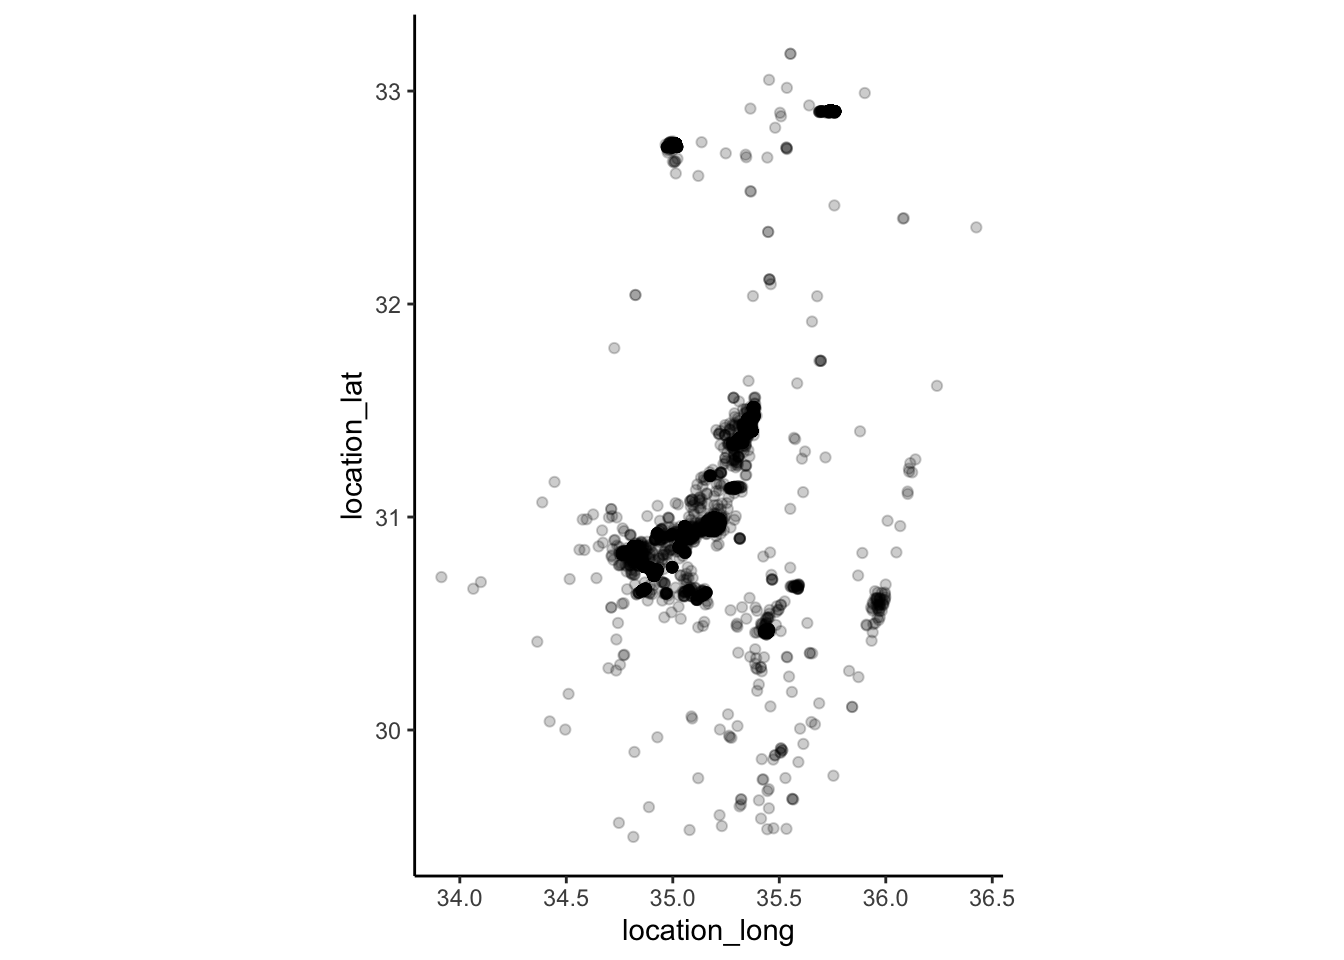
\includegraphics{arrivalAtCarcasses_files/figure-latex/unnamed-chunk-4-1.pdf}
Okay, that's not very informative, as expected. Let's split this by day
and just look at one day's sequence.

\begin{Shaded}
\begin{Highlighting}[]
\NormalTok{accDays }\OtherTok{\textless{}{-}} \FunctionTok{lapply}\NormalTok{(trackDays, }\ControlFlowTok{function}\NormalTok{(x)\{}
\NormalTok{  x }\SpecialCharTok{\%\textgreater{}\%}\NormalTok{ dplyr}\SpecialCharTok{::}\FunctionTok{select}\NormalTok{(dateOnly, timestamp, }\FunctionTok{contains}\NormalTok{(}\StringTok{"acceleration\_"}\NormalTok{)) }\SpecialCharTok{\%\textgreater{}\%}
    \FunctionTok{pivot\_longer}\NormalTok{(}\AttributeTok{cols =} \FunctionTok{contains}\NormalTok{(}\StringTok{"acceleration\_"}\NormalTok{), }\AttributeTok{names\_to =} \StringTok{"axis"}\NormalTok{, }\AttributeTok{values\_to =} \StringTok{"acceleration"}\NormalTok{) }\SpecialCharTok{\%\textgreater{}\%}
    \FunctionTok{mutate}\NormalTok{(}\AttributeTok{axis =} \FunctionTok{str\_remove}\NormalTok{(axis, }\StringTok{"acceleration\_raw\_"}\NormalTok{))}
\NormalTok{\})}
\end{Highlighting}
\end{Shaded}

\begin{Shaded}
\begin{Highlighting}[]
\NormalTok{randomDay }\OtherTok{\textless{}{-}} \FunctionTok{sample}\NormalTok{(}\DecValTok{1}\SpecialCharTok{:}\FunctionTok{length}\NormalTok{(accDays), }\AttributeTok{size =} \DecValTok{1}\NormalTok{)}

\NormalTok{accDays[[randomDay]] }\SpecialCharTok{\%\textgreater{}\%}
  \FunctionTok{ggplot}\NormalTok{(}\FunctionTok{aes}\NormalTok{(}\AttributeTok{x =}\NormalTok{ timestamp, }\AttributeTok{y =}\NormalTok{ acceleration, }\AttributeTok{col =}\NormalTok{ axis))}\SpecialCharTok{+}
  \FunctionTok{geom\_line}\NormalTok{()}
\end{Highlighting}
\end{Shaded}

\includegraphics{arrivalAtCarcasses_files/figure-latex/unnamed-chunk-6-1.pdf}
Okay, this is kind of cool. But I'm not good enough at interpreting
accelerometer data to know for sure how to read this.

\hypertarget{speed-and-altitude}{%
\subsubsection{Speed and altitude}\label{speed-and-altitude}}

What about speed and altitude? Can the combination of those tell us what
we need to know?

\begin{Shaded}
\begin{Highlighting}[]
\NormalTok{randomDay }\OtherTok{\textless{}{-}} \FunctionTok{sample}\NormalTok{(}\DecValTok{1}\SpecialCharTok{:}\FunctionTok{length}\NormalTok{(accDays), }\AttributeTok{size =} \DecValTok{1}\NormalTok{)}
\NormalTok{speed }\OtherTok{\textless{}{-}}\NormalTok{ trackDays[[randomDay]] }\SpecialCharTok{\%\textgreater{}\%}
  \FunctionTok{ggplot}\NormalTok{(}\FunctionTok{aes}\NormalTok{(}\AttributeTok{x =}\NormalTok{ timestamp, }\AttributeTok{y =}\NormalTok{ ground\_speed))}\SpecialCharTok{+}
  \FunctionTok{geom\_line}\NormalTok{()}
\NormalTok{speed}
\end{Highlighting}
\end{Shaded}

\includegraphics{arrivalAtCarcasses_files/figure-latex/unnamed-chunk-7-1.pdf}

\begin{Shaded}
\begin{Highlighting}[]
\NormalTok{altitude }\OtherTok{\textless{}{-}}\NormalTok{ trackDays[[randomDay]] }\SpecialCharTok{\%\textgreater{}\%}
  \FunctionTok{ggplot}\NormalTok{(}\FunctionTok{aes}\NormalTok{(}\AttributeTok{x =}\NormalTok{ timestamp, }\AttributeTok{y =}\NormalTok{ height\_above\_msl))}\SpecialCharTok{+}
  \FunctionTok{geom\_line}\NormalTok{()}
\NormalTok{altitude}
\end{Highlighting}
\end{Shaded}

\includegraphics{arrivalAtCarcasses_files/figure-latex/unnamed-chunk-7-2.pdf}

\hypertarget{relative-altitude}{%
\subsubsection{Relative altitude}\label{relative-altitude}}

In order for this to make any sense at all, we need to cross-reference
these measurements with elevation data for Israel. We can obtain this
using the \texttt{elevatr} package.

\begin{Shaded}
\begin{Highlighting}[]
\CommentTok{\# Add sunrise and sunset information using suncalc}
\DocumentationTok{\#\# first let\textquotesingle{}s get the mean lat and long for the current track}
\NormalTok{meanLat }\OtherTok{\textless{}{-}} \FunctionTok{mean}\NormalTok{(track}\SpecialCharTok{$}\NormalTok{location\_lat)}
\NormalTok{meanLong }\OtherTok{\textless{}{-}} \FunctionTok{mean}\NormalTok{(track}\SpecialCharTok{$}\NormalTok{location\_long)}
\NormalTok{dates }\OtherTok{\textless{}{-}} \FunctionTok{seq}\NormalTok{(}\AttributeTok{from =} \FunctionTok{min}\NormalTok{(track}\SpecialCharTok{$}\NormalTok{dateOnly), }\AttributeTok{to =} \FunctionTok{max}\NormalTok{(track}\SpecialCharTok{$}\NormalTok{dateOnly), }\AttributeTok{by =} \StringTok{"1 day"}\NormalTok{)}
\NormalTok{sunriseSunset }\OtherTok{\textless{}{-}}\NormalTok{ suncalc}\SpecialCharTok{::}\FunctionTok{getSunlightTimes}\NormalTok{(}\AttributeTok{date =}\NormalTok{ dates, }\AttributeTok{lat =}\NormalTok{ meanLat, }\AttributeTok{lon =}\NormalTok{ meanLong, }\AttributeTok{keep =} \FunctionTok{c}\NormalTok{(}\StringTok{"sunrise"}\NormalTok{, }\StringTok{"sunset"}\NormalTok{)) }\SpecialCharTok{\%\textgreater{}\%}
\NormalTok{  dplyr}\SpecialCharTok{::}\FunctionTok{select}\NormalTok{(}\StringTok{"dateOnly"} \OtherTok{=}\NormalTok{ date, sunrise, sunset)}
\NormalTok{track }\OtherTok{\textless{}{-}}\NormalTok{ track }\SpecialCharTok{\%\textgreater{}\%}
  \FunctionTok{left\_join}\NormalTok{(sunriseSunset, }\AttributeTok{by =} \StringTok{"dateOnly"}\NormalTok{)}

\CommentTok{\# Make it an sf object and add elevation}
\NormalTok{trackSF }\OtherTok{\textless{}{-}}\NormalTok{ track }\SpecialCharTok{\%\textgreater{}\%}
\NormalTok{  sf}\SpecialCharTok{::}\FunctionTok{st\_as\_sf}\NormalTok{(., }\AttributeTok{coords =} \FunctionTok{c}\NormalTok{(}\StringTok{"location\_long"}\NormalTok{, }\StringTok{"location\_lat"}\NormalTok{), }\AttributeTok{crs =} \StringTok{"WGS84"}\NormalTok{)}
\NormalTok{elevs }\OtherTok{\textless{}{-}}\NormalTok{ elevatr}\SpecialCharTok{::}\FunctionTok{get\_elev\_raster}\NormalTok{(trackSF, }\AttributeTok{z =} \DecValTok{10}\NormalTok{) }
\end{Highlighting}
\end{Shaded}

\begin{verbatim}
## Mosaicing & Projecting
\end{verbatim}

\begin{verbatim}
## Note: Elevation units are in meters.
\end{verbatim}

\begin{Shaded}
\begin{Highlighting}[]
\NormalTok{trackSF}\SpecialCharTok{$}\NormalTok{groundElev }\OtherTok{\textless{}{-}}\NormalTok{ raster}\SpecialCharTok{::}\FunctionTok{extract}\NormalTok{(}\AttributeTok{x =}\NormalTok{ elevs, }\AttributeTok{y =}\NormalTok{ trackSF)}
\NormalTok{trackSF }\OtherTok{\textless{}{-}}\NormalTok{ trackSF }\SpecialCharTok{\%\textgreater{}\%}
  \FunctionTok{mutate}\NormalTok{(}\AttributeTok{height\_above\_ground =}\NormalTok{ height\_above\_msl }\SpecialCharTok{{-}}\NormalTok{ groundElev)}

\CommentTok{\# let\textquotesingle{}s set anything below 0 to 0.}
\NormalTok{trackSF }\OtherTok{\textless{}{-}}\NormalTok{ trackSF }\SpecialCharTok{\%\textgreater{}\%}
  \FunctionTok{mutate}\NormalTok{(}\AttributeTok{height\_above\_ground =} \FunctionTok{case\_when}\NormalTok{(height\_above\_ground }\SpecialCharTok{\textless{}} \DecValTok{0} \SpecialCharTok{\textasciitilde{}} \DecValTok{0}\NormalTok{,}
                                         \ConstantTok{TRUE} \SpecialCharTok{\textasciitilde{}}\NormalTok{ height\_above\_ground))}

\NormalTok{trackDaysSF }\OtherTok{\textless{}{-}}\NormalTok{ trackSF }\SpecialCharTok{\%\textgreater{}\%}
  \FunctionTok{group\_by}\NormalTok{(dateOnly) }\SpecialCharTok{\%\textgreater{}\%}
  \FunctionTok{group\_split}\NormalTok{(}\AttributeTok{.keep =} \ConstantTok{TRUE}\NormalTok{)}
\end{Highlighting}
\end{Shaded}

\hypertarget{speedrelative-altitude-plots}{%
\paragraph{Speed/relative altitude
plots}\label{speedrelative-altitude-plots}}

Now let's re-do the speed and altitude plots, using altitude above
ground:

\begin{Shaded}
\begin{Highlighting}[]
\CommentTok{\# create rectangles to add to ggplot, assuming the dataset has the "sunrise" and "sunset" and "timestamp" columns.}
\NormalTok{sunriseSunsetBars }\OtherTok{\textless{}{-}} \FunctionTok{list}\NormalTok{(}\FunctionTok{geom\_rect}\NormalTok{(}\FunctionTok{aes}\NormalTok{(}\AttributeTok{xmin =} \FunctionTok{min}\NormalTok{(timestamp),}
                                        \AttributeTok{xmax =} \FunctionTok{min}\NormalTok{(sunrise),}
                                        \AttributeTok{ymin =} \SpecialCharTok{{-}}\ConstantTok{Inf}\NormalTok{,}
                                        \AttributeTok{ymax =} \ConstantTok{Inf}\NormalTok{), }\AttributeTok{alpha =} \FloatTok{0.003}\NormalTok{),}
                          \FunctionTok{geom\_rect}\NormalTok{(}\FunctionTok{aes}\NormalTok{(}\AttributeTok{xmin =} \FunctionTok{max}\NormalTok{(sunset),}
                                        \AttributeTok{xmax =} \FunctionTok{max}\NormalTok{(timestamp),}
                                        \AttributeTok{ymin =} \SpecialCharTok{{-}}\ConstantTok{Inf}\NormalTok{,}
                                        \AttributeTok{ymax =} \ConstantTok{Inf}\NormalTok{), }\AttributeTok{alpha =} \FloatTok{0.003}\NormalTok{))}

\NormalTok{randomDay }\OtherTok{\textless{}{-}} \FunctionTok{sample}\NormalTok{(}\DecValTok{1}\SpecialCharTok{:}\FunctionTok{length}\NormalTok{(trackDaysSF), }\AttributeTok{size =} \DecValTok{1}\NormalTok{)}

\NormalTok{altitude }\OtherTok{\textless{}{-}}\NormalTok{ trackDaysSF[[randomDay]] }\SpecialCharTok{\%\textgreater{}\%}
  \FunctionTok{mutate}\NormalTok{(}\AttributeTok{height\_above\_msl =} \FunctionTok{case\_when}\NormalTok{(height\_above\_msl }\SpecialCharTok{\textless{}}\NormalTok{ groundElev }\SpecialCharTok{\textasciitilde{}}\NormalTok{ groundElev,}
                                      \ConstantTok{TRUE} \SpecialCharTok{\textasciitilde{}}\NormalTok{ height\_above\_msl)) }\SpecialCharTok{\%\textgreater{}\%}
  \FunctionTok{ggplot}\NormalTok{(}\FunctionTok{aes}\NormalTok{(}\AttributeTok{x =}\NormalTok{ timestamp, }\AttributeTok{y =}\NormalTok{ height\_above\_msl))}\SpecialCharTok{+}
  \FunctionTok{geom\_area}\NormalTok{(}\FunctionTok{aes}\NormalTok{(}\AttributeTok{y =}\NormalTok{ groundElev), }\AttributeTok{fill =} \StringTok{"\#996633"}\NormalTok{)}\SpecialCharTok{+}
  \FunctionTok{geom\_line}\NormalTok{(}\AttributeTok{alpha =} \FloatTok{0.5}\NormalTok{)}\SpecialCharTok{+}
  \FunctionTok{geom\_point}\NormalTok{(}\FunctionTok{aes}\NormalTok{(}\AttributeTok{col =}\NormalTok{ ground\_speed), }\AttributeTok{size =} \DecValTok{3}\NormalTok{)}\SpecialCharTok{+}
  \FunctionTok{scale\_color\_viridis\_c}\NormalTok{()}\SpecialCharTok{+}
  \FunctionTok{ylab}\NormalTok{(}\StringTok{"Elevation (m)"}\NormalTok{)}\SpecialCharTok{+}
  \FunctionTok{xlab}\NormalTok{(}\StringTok{"Time"}\NormalTok{)}\SpecialCharTok{+}
  \FunctionTok{theme\_minimal}\NormalTok{()}\SpecialCharTok{+}
\NormalTok{  sunriseSunsetBars}
\NormalTok{altitude}
\end{Highlighting}
\end{Shaded}

\includegraphics{arrivalAtCarcasses_files/figure-latex/unnamed-chunk-9-1.pdf}

\hypertarget{known-feeding-events}{%
\subsection{KNOWN FEEDING EVENTS}\label{known-feeding-events}}

\hypertarget{feeding-event-data}{%
\subsubsection{Feeding event data}\label{feeding-event-data}}

Read in the feeding event data (this is the most updated version we
have; should work on getting more info from more recent feeding events.)

\hypertarget{sunrisesunset-daynight-to-datannot}{%
\paragraph{Sunrise/sunset, day/night to
datAnnot}\label{sunrisesunset-daynight-to-datannot}}

\begin{Shaded}
\begin{Highlighting}[]
\CommentTok{\# using the mean values of lat and long for this dataset, which may not be perfect but it\textquotesingle{}s fairly decent.}
\NormalTok{meanLat }\OtherTok{\textless{}{-}} \FunctionTok{mean}\NormalTok{(datAnnot}\SpecialCharTok{$}\NormalTok{location\_lat)}
\NormalTok{meanLong }\OtherTok{\textless{}{-}} \FunctionTok{mean}\NormalTok{(datAnnot}\SpecialCharTok{$}\NormalTok{location\_long)}

\CommentTok{\# Add sunrise/sunset information for each day, and use it to calculate whether each point takes place during day or night.}
\NormalTok{sunriseSunset }\OtherTok{\textless{}{-}}\NormalTok{ suncalc}\SpecialCharTok{::}\FunctionTok{getSunlightTimes}\NormalTok{(}\AttributeTok{date =} \FunctionTok{unique}\NormalTok{(datAnnot}\SpecialCharTok{$}\NormalTok{dateOnly), }\AttributeTok{lat =}\NormalTok{ meanLat, }\AttributeTok{lon =}\NormalTok{ meanLong, }\AttributeTok{keep =} \FunctionTok{c}\NormalTok{(}\StringTok{"sunrise"}\NormalTok{, }\StringTok{"sunset"}\NormalTok{)) }\SpecialCharTok{\%\textgreater{}\%}
\NormalTok{  dplyr}\SpecialCharTok{::}\FunctionTok{select}\NormalTok{(}\StringTok{"dateOnly"} \OtherTok{=}\NormalTok{ date, sunrise, sunset)}

\NormalTok{sunsetSunrise }\OtherTok{\textless{}{-}}\NormalTok{ sunriseSunset }\SpecialCharTok{\%\textgreater{}\%}
\NormalTok{  dplyr}\SpecialCharTok{::}\FunctionTok{select}\NormalTok{(sunset, sunrise) }\SpecialCharTok{\%\textgreater{}\%}
  \FunctionTok{mutate}\NormalTok{(}\AttributeTok{sunrise =} \FunctionTok{lead}\NormalTok{(sunrise))}

\NormalTok{datAnnot }\OtherTok{\textless{}{-}}\NormalTok{ datAnnot }\SpecialCharTok{\%\textgreater{}\%}
  \FunctionTok{left\_join}\NormalTok{(sunriseSunset, }\AttributeTok{by =} \StringTok{"dateOnly"}\NormalTok{) }\SpecialCharTok{\%\textgreater{}\%}
  \FunctionTok{mutate}\NormalTok{(}\AttributeTok{dayNight =} \FunctionTok{case\_when}\NormalTok{(timestamp }\SpecialCharTok{\textgreater{}=}\NormalTok{ sunrise }\SpecialCharTok{\&}\NormalTok{ timestamp }\SpecialCharTok{\textless{}=}\NormalTok{ sunset }\SpecialCharTok{\textasciitilde{}} \StringTok{"day"}\NormalTok{,}
                              \ConstantTok{TRUE} \SpecialCharTok{\textasciitilde{}} \StringTok{"night"}\NormalTok{)) }\SpecialCharTok{\%\textgreater{}\%}
\NormalTok{  dplyr}\SpecialCharTok{::}\FunctionTok{select}\NormalTok{(}\SpecialCharTok{{-}}\FunctionTok{c}\NormalTok{(}\StringTok{"sunrise"}\NormalTok{, }\StringTok{"sunset"}\NormalTok{)) }\SpecialCharTok{\%\textgreater{}\%}
  \FunctionTok{mutate}\NormalTok{(}\AttributeTok{dayNight =} \FunctionTok{factor}\NormalTok{(dayNight))}
\end{Highlighting}
\end{Shaded}

\begin{Shaded}
\begin{Highlighting}[]
\NormalTok{feedEvents }\OtherTok{\textless{}{-}} \FunctionTok{read.csv}\NormalTok{(}\StringTok{"data/feeding\_station\_south\_data.xlsx {-} Sheet1.csv"}\NormalTok{)}
\CommentTok{\# add datetime}
\NormalTok{feedEvents }\OtherTok{\textless{}{-}}\NormalTok{ feedEvents }\SpecialCharTok{\%\textgreater{}\%}
  \FunctionTok{mutate}\NormalTok{(}\AttributeTok{datetime =}\NormalTok{ lubridate}\SpecialCharTok{::}\FunctionTok{mdy\_hms}\NormalTok{(Timestamp)) }\SpecialCharTok{\%\textgreater{}\%}
\NormalTok{  dplyr}\SpecialCharTok{::}\FunctionTok{select}\NormalTok{(}\SpecialCharTok{{-}}\NormalTok{Timestamp)}

\CommentTok{\# Subset to only include feeding events that occurred within the time range of this dataset}
\NormalTok{min }\OtherTok{\textless{}{-}} \FunctionTok{min}\NormalTok{(datAnnot}\SpecialCharTok{$}\NormalTok{timestamp)}
\NormalTok{max }\OtherTok{\textless{}{-}} \FunctionTok{max}\NormalTok{(datAnnot}\SpecialCharTok{$}\NormalTok{timestamp)}
\NormalTok{feedEvents }\OtherTok{\textless{}{-}}\NormalTok{ feedEvents }\SpecialCharTok{\%\textgreater{}\%}
  \FunctionTok{filter}\NormalTok{(datetime }\SpecialCharTok{\textgreater{}=}\NormalTok{ min }\SpecialCharTok{\&}\NormalTok{ datetime }\SpecialCharTok{\textless{}=}\NormalTok{ max)}
\FunctionTok{nrow}\NormalTok{(feedEvents)}
\end{Highlighting}
\end{Shaded}

\begin{verbatim}
## [1] 75
\end{verbatim}

\begin{Shaded}
\begin{Highlighting}[]
\FunctionTok{head}\NormalTok{(feedEvents)}
\end{Highlighting}
\end{Shaded}

\begin{verbatim}
##   feeding_date feeding_time death_of_carcass_known hours_since_death
## 1    8/30/2020  11:30:00 AM                     no                24
## 2     9/1/2020   2:15:00 PM                     no                24
## 3     9/4/2020  10:55:00 AM                     no                24
## 4     9/6/2020  11:10:00 AM                     no                24
## 5     9/7/2020   9:20:00 AM                     no                24
## 6    9/10/2020   1:00:00 PM                     no                12
##                   area   feeding_station         carcass_type weight_of_food
## 1      SdeBoker_Hatira       Tzaror_trap donkey, sheep, horse            350
## 2 Small_and_Big_crater Small_crater_view          ibex, sheep            130
## 3      SdeBoker_Hatira       Tzaror_trap          sheep, calf            310
## 4  South_Judean_desert     Ben_Yair_view           sheep, cow            660
## 5      SdeBoker_Hatira          Antenas                   cow            600
## 6         Ramon_crater            Kaolin            calf, cow            540
##   no_of_carcasses origin_carcass        ranger              remarks
## 1               3         בדואים      עין עבדת   לטובת לכידת נשרים 
## 2               3        הר הנגב    עודד צעירי הונח גם עוף מסוג אמו
## 3               7           מקרר      עין עבדת  לטובת לכידות נשרים 
## 4               2       טללי שדה ג'מיל אל אטרש                     
## 5               1       טללי שדה יבגני קמינסקי                     
## 6               2    קיבוץ צאלים   ידידה שמואל       הצבת שוקת מים 
##              datetime
## 1 2020-08-30 10:56:53
## 2 2020-09-01 13:16:41
## 3 2020-09-04 09:55:39
## 4 2020-09-06 10:13:52
## 5 2020-09-07 08:40:28
## 6 2020-09-10 12:26:09
\end{verbatim}

\begin{Shaded}
\begin{Highlighting}[]
\FunctionTok{table}\NormalTok{(feedEvents}\SpecialCharTok{$}\NormalTok{area)}
\end{Highlighting}
\end{Shaded}

\begin{verbatim}
## 
##         Arava_valley         Ramon_crater      SdeBoker_Hatira 
##                    7                   11                   28 
## Small_and_Big_crater  South_Judean_desert     West_negev_sands 
##                   22                    6                    1
\end{verbatim}

\hypertarget{feeding-station-locations}{%
\subsubsection{Feeding station
locations}\label{feeding-station-locations}}

Okay, now that we have that data, we critically need access to the
feeding station data so that we can match these carcass drops to
lat/long.

\begin{Shaded}
\begin{Highlighting}[]
\NormalTok{feedingStations }\OtherTok{\textless{}{-}} \FunctionTok{read.csv}\NormalTok{(}\StringTok{"data/feeding\_station\_south\_coordinates.xlsx {-} Sheet1.csv"}\NormalTok{)}
\FunctionTok{head}\NormalTok{(feedingStations)}
\end{Highlighting}
\end{Shaded}

\begin{verbatim}
##   Feeding_station Active_Not_active  ITM_E  ITM_N        lat    long
## 1        Antenas                yes 178602 538292    30.9349 34.7770
## 2      Gorni_hill               yes 228080 580867 31.319568  35.2951
## 3          Golhan               yes 203938 533826    30.8952 35.0422
## 4          Daroch               yes 184290 530148    30.8616 34.8368
## 5     Camus_south               yes 205225 540429    30.9548 35.0556
## 6   Hahalak_mount               yes 203447 530437    30.8646 35.0371
\end{verbatim}

\begin{Shaded}
\begin{Highlighting}[]
\CommentTok{\# Are we going to be able to join these by name? I am not optimistic...}
\NormalTok{feedEvents}\SpecialCharTok{$}\NormalTok{feeding\_station }\SpecialCharTok{\%in\%}\NormalTok{ feedingStations}\SpecialCharTok{$}\NormalTok{Feeding\_station }\CommentTok{\# awesome!!! oh my gosh.}
\end{Highlighting}
\end{Shaded}

\begin{verbatim}
##  [1] TRUE TRUE TRUE TRUE TRUE TRUE TRUE TRUE TRUE TRUE TRUE TRUE TRUE TRUE TRUE
## [16] TRUE TRUE TRUE TRUE TRUE TRUE TRUE TRUE TRUE TRUE TRUE TRUE TRUE TRUE TRUE
## [31] TRUE TRUE TRUE TRUE TRUE TRUE TRUE TRUE TRUE TRUE TRUE TRUE TRUE TRUE TRUE
## [46] TRUE TRUE TRUE TRUE TRUE TRUE TRUE TRUE TRUE TRUE TRUE TRUE TRUE TRUE TRUE
## [61] TRUE TRUE TRUE TRUE TRUE TRUE TRUE TRUE TRUE TRUE TRUE TRUE TRUE TRUE TRUE
\end{verbatim}

\begin{Shaded}
\begin{Highlighting}[]
\CommentTok{\# okay, let\textquotesingle{}s join the coordinates}
\NormalTok{feedEvents }\OtherTok{\textless{}{-}}\NormalTok{ feedEvents }\SpecialCharTok{\%\textgreater{}\%}
  \FunctionTok{left\_join}\NormalTok{(feedingStations }\SpecialCharTok{\%\textgreater{}\%}
\NormalTok{              dplyr}\SpecialCharTok{::}\FunctionTok{select}\NormalTok{(Feeding\_station, lat, long),}
            \AttributeTok{by =} \FunctionTok{c}\NormalTok{(}\StringTok{"feeding\_station"} \OtherTok{=} \StringTok{"Feeding\_station"}\NormalTok{)) }\SpecialCharTok{\%\textgreater{}\%}
  \FunctionTok{mutate}\NormalTok{(}\AttributeTok{lat =} \FunctionTok{as.numeric}\NormalTok{(lat),}
         \AttributeTok{long =} \FunctionTok{as.numeric}\NormalTok{(long))}
\end{Highlighting}
\end{Shaded}

\begin{verbatim}
## Warning in mask$eval_all_mutate(quo): NAs introduced by coercion

## Warning in mask$eval_all_mutate(quo): NAs introduced by coercion
\end{verbatim}

\begin{Shaded}
\begin{Highlighting}[]
\FunctionTok{head}\NormalTok{(feedEvents)}
\end{Highlighting}
\end{Shaded}

\begin{verbatim}
##   feeding_date feeding_time death_of_carcass_known hours_since_death
## 1    8/30/2020  11:30:00 AM                     no                24
## 2     9/1/2020   2:15:00 PM                     no                24
## 3     9/4/2020  10:55:00 AM                     no                24
## 4     9/6/2020  11:10:00 AM                     no                24
## 5     9/7/2020   9:20:00 AM                     no                24
## 6    9/10/2020   1:00:00 PM                     no                12
##                   area   feeding_station         carcass_type weight_of_food
## 1      SdeBoker_Hatira       Tzaror_trap donkey, sheep, horse            350
## 2 Small_and_Big_crater Small_crater_view          ibex, sheep            130
## 3      SdeBoker_Hatira       Tzaror_trap          sheep, calf            310
## 4  South_Judean_desert     Ben_Yair_view           sheep, cow            660
## 5      SdeBoker_Hatira          Antenas                   cow            600
## 6         Ramon_crater            Kaolin            calf, cow            540
##   no_of_carcasses origin_carcass        ranger              remarks
## 1               3         בדואים      עין עבדת   לטובת לכידת נשרים 
## 2               3        הר הנגב    עודד צעירי הונח גם עוף מסוג אמו
## 3               7           מקרר      עין עבדת  לטובת לכידות נשרים 
## 4               2       טללי שדה ג'מיל אל אטרש                     
## 5               1       טללי שדה יבגני קמינסקי                     
## 6               2    קיבוץ צאלים   ידידה שמואל       הצבת שוקת מים 
##              datetime     lat    long
## 1 2020-08-30 10:56:53 30.8615 34.8136
## 2 2020-09-01 13:16:41 30.9490 35.1508
## 3 2020-09-04 09:55:39 30.8615 34.8136
## 4 2020-09-06 10:13:52 31.3321 35.3305
## 5 2020-09-07 08:40:28 30.9349 34.7770
## 6 2020-09-10 12:26:09      NA 34.8491
\end{verbatim}

\begin{Shaded}
\begin{Highlighting}[]
\CommentTok{\# Remove any missing values. Later, will need to ask Gideon why these coordinates are missing, and see what we can do about it. But for now, this is just a proof of concept.}
\NormalTok{feedEvents }\OtherTok{\textless{}{-}}\NormalTok{ feedEvents }\SpecialCharTok{\%\textgreater{}\%}
  \FunctionTok{filter}\NormalTok{(}\SpecialCharTok{!}\FunctionTok{is.na}\NormalTok{(lat) }\SpecialCharTok{\&} \SpecialCharTok{!}\FunctionTok{is.na}\NormalTok{(long))}

\CommentTok{\# Now make it an sf object}
\NormalTok{feedEvents }\OtherTok{\textless{}{-}}\NormalTok{ feedEvents }\SpecialCharTok{\%\textgreater{}\%}
\NormalTok{  sf}\SpecialCharTok{::}\FunctionTok{st\_as\_sf}\NormalTok{(., }\AttributeTok{coords =} \FunctionTok{c}\NormalTok{(}\StringTok{"long"}\NormalTok{, }\StringTok{"lat"}\NormalTok{), }\AttributeTok{remove =} \ConstantTok{FALSE}\NormalTok{) }\SpecialCharTok{\%\textgreater{}\%}
\NormalTok{  sf}\SpecialCharTok{::}\FunctionTok{st\_set\_crs}\NormalTok{(}\StringTok{"WGS84"}\NormalTok{) }\SpecialCharTok{\%\textgreater{}\%}
\NormalTok{  dplyr}\SpecialCharTok{::}\FunctionTok{select}\NormalTok{(}\SpecialCharTok{{-}}\FunctionTok{c}\NormalTok{(death\_of\_carcass\_known, hours\_since\_death, origin\_carcass, ranger, remarks))}
\end{Highlighting}
\end{Shaded}

\hypertarget{exploratory-mapping}{%
\subsubsection{Exploratory mapping}\label{exploratory-mapping}}

\begin{Shaded}
\begin{Highlighting}[]
\NormalTok{mask }\OtherTok{\textless{}{-}} \FunctionTok{suppressMessages}\NormalTok{(sf}\SpecialCharTok{::}\FunctionTok{st\_read}\NormalTok{(}\StringTok{"data/CutOffRegion.kml"}\NormalTok{))}
\end{Highlighting}
\end{Shaded}

\begin{verbatim}
## Reading layer `CutOffRegion.kml' from data source 
##   `/Users/kaijagahmpersonalprojects/Desktop/dataExploration/data/CutOffRegion.kml' 
##   using driver `KML'
## Simple feature collection with 1 feature and 2 fields
## Geometry type: POLYGON
## Dimension:     XYZ
## Bounding box:  xmin: 33.46685 ymin: 29.47732 xmax: 36.72913 ymax: 33.51767
## z_range:       zmin: 0 zmax: 0
## Geodetic CRS:  WGS 84
\end{verbatim}

\begin{Shaded}
\begin{Highlighting}[]
\NormalTok{datMasked }\OtherTok{\textless{}{-}}\NormalTok{ vultureUtils}\SpecialCharTok{::}\FunctionTok{maskData}\NormalTok{(}\AttributeTok{dataset =}\NormalTok{ datAnnot, }\AttributeTok{mask =}\NormalTok{ mask, }\AttributeTok{longCol =} \StringTok{"location\_long.1"}\NormalTok{, }\AttributeTok{latCol =} \StringTok{"location\_lat.1"}\NormalTok{, }\AttributeTok{crs =} \StringTok{"WGS84"}\NormalTok{)}
\end{Highlighting}
\end{Shaded}

\begin{verbatim}
## st_as_s2(): dropping Z and/or M coordinate
\end{verbatim}

\begin{Shaded}
\begin{Highlighting}[]
\CommentTok{\# Get bounding box}
\NormalTok{lon }\OtherTok{\textless{}{-}} \FunctionTok{range}\NormalTok{(datMasked}\SpecialCharTok{$}\NormalTok{location\_long)}
\NormalTok{lat }\OtherTok{\textless{}{-}} \FunctionTok{range}\NormalTok{(datMasked}\SpecialCharTok{$}\NormalTok{location\_lat)}

\NormalTok{map }\OtherTok{\textless{}{-}}\NormalTok{ ggmap}\SpecialCharTok{::}\FunctionTok{get\_stamenmap}\NormalTok{(}\AttributeTok{bbox =} \FunctionTok{c}\NormalTok{(lon[}\DecValTok{1}\NormalTok{], lat[}\DecValTok{1}\NormalTok{], lon[}\DecValTok{2}\NormalTok{], lat[}\DecValTok{2}\NormalTok{]), }\AttributeTok{zoom =} \DecValTok{7}\NormalTok{, }\AttributeTok{maptype =} \StringTok{"terrain{-}background"}\NormalTok{)}
\end{Highlighting}
\end{Shaded}

\begin{verbatim}
## Source : http://tile.stamen.com/terrain-background/7/75/51.png
\end{verbatim}

\begin{verbatim}
## Source : http://tile.stamen.com/terrain-background/7/76/51.png
\end{verbatim}

\begin{verbatim}
## Source : http://tile.stamen.com/terrain-background/7/75/52.png
\end{verbatim}

\begin{verbatim}
## Source : http://tile.stamen.com/terrain-background/7/76/52.png
\end{verbatim}

\begin{verbatim}
## Source : http://tile.stamen.com/terrain-background/7/75/53.png
\end{verbatim}

\begin{verbatim}
## Source : http://tile.stamen.com/terrain-background/7/76/53.png
\end{verbatim}

\begin{Shaded}
\begin{Highlighting}[]
\NormalTok{map}
\end{Highlighting}
\end{Shaded}

\begin{verbatim}
## 428x252 terrain-background map image from Stamen Maps. 
## See ?ggmap to plot it.
\end{verbatim}

\begin{Shaded}
\begin{Highlighting}[]
\NormalTok{test }\OtherTok{\textless{}{-}}\NormalTok{ datMasked[}\DecValTok{1}\SpecialCharTok{:}\DecValTok{100}\NormalTok{,] }\SpecialCharTok{\%\textgreater{}\%}
\NormalTok{  sf}\SpecialCharTok{::}\FunctionTok{st\_set\_crs}\NormalTok{(}\StringTok{"WGS84"}\NormalTok{)}

\CommentTok{\# Get one individual}
\NormalTok{test }\OtherTok{\textless{}{-}}\NormalTok{ datMasked }\SpecialCharTok{\%\textgreater{}\%}
  \FunctionTok{filter}\NormalTok{(trackId }\SpecialCharTok{==} \StringTok{"T61w"}\NormalTok{)}

\CommentTok{\# Get bounding box for this indiv}
\NormalTok{lon }\OtherTok{\textless{}{-}} \FunctionTok{range}\NormalTok{(test}\SpecialCharTok{$}\NormalTok{location\_long)}
\NormalTok{lat }\OtherTok{\textless{}{-}} \FunctionTok{range}\NormalTok{(test}\SpecialCharTok{$}\NormalTok{location\_lat)}

\NormalTok{map }\OtherTok{\textless{}{-}}\NormalTok{ ggmap}\SpecialCharTok{::}\FunctionTok{get\_stamenmap}\NormalTok{(}\AttributeTok{bbox =} \FunctionTok{c}\NormalTok{(lon[}\DecValTok{1}\NormalTok{], lat[}\DecValTok{1}\NormalTok{], lon[}\DecValTok{2}\NormalTok{], lat[}\DecValTok{2}\NormalTok{]), }\AttributeTok{zoom =} \DecValTok{10}\NormalTok{, }\AttributeTok{maptype =} \StringTok{"terrain{-}background"}\NormalTok{)}
\end{Highlighting}
\end{Shaded}

\begin{verbatim}
## Source : http://tile.stamen.com/terrain-background/10/611/413.png
\end{verbatim}

\begin{verbatim}
## Source : http://tile.stamen.com/terrain-background/10/611/414.png
\end{verbatim}

\begin{Shaded}
\begin{Highlighting}[]
\CommentTok{\# Make the map}
\FunctionTok{ggmap}\NormalTok{(map)}\SpecialCharTok{+}
  \FunctionTok{geom\_point}\NormalTok{(}\AttributeTok{data =}\NormalTok{ test, }\FunctionTok{aes}\NormalTok{(}\AttributeTok{x =}\NormalTok{ location\_long}\FloatTok{.1}\NormalTok{, }\AttributeTok{y =}\NormalTok{ location\_lat}\FloatTok{.1}\NormalTok{, }\AttributeTok{col =}\NormalTok{ ground\_speed), }\AttributeTok{size =} \FloatTok{0.2}\NormalTok{)}\SpecialCharTok{+}
  \FunctionTok{geom\_path}\NormalTok{(}\AttributeTok{data =}\NormalTok{ test, }\FunctionTok{aes}\NormalTok{(}\AttributeTok{x =}\NormalTok{ location\_long}\FloatTok{.1}\NormalTok{, }\AttributeTok{y =}\NormalTok{ location\_lat}\FloatTok{.1}\NormalTok{), }\AttributeTok{size =} \FloatTok{0.02}\NormalTok{)}\SpecialCharTok{+}
  \FunctionTok{scale\_color\_viridis\_c}\NormalTok{()}
\end{Highlighting}
\end{Shaded}

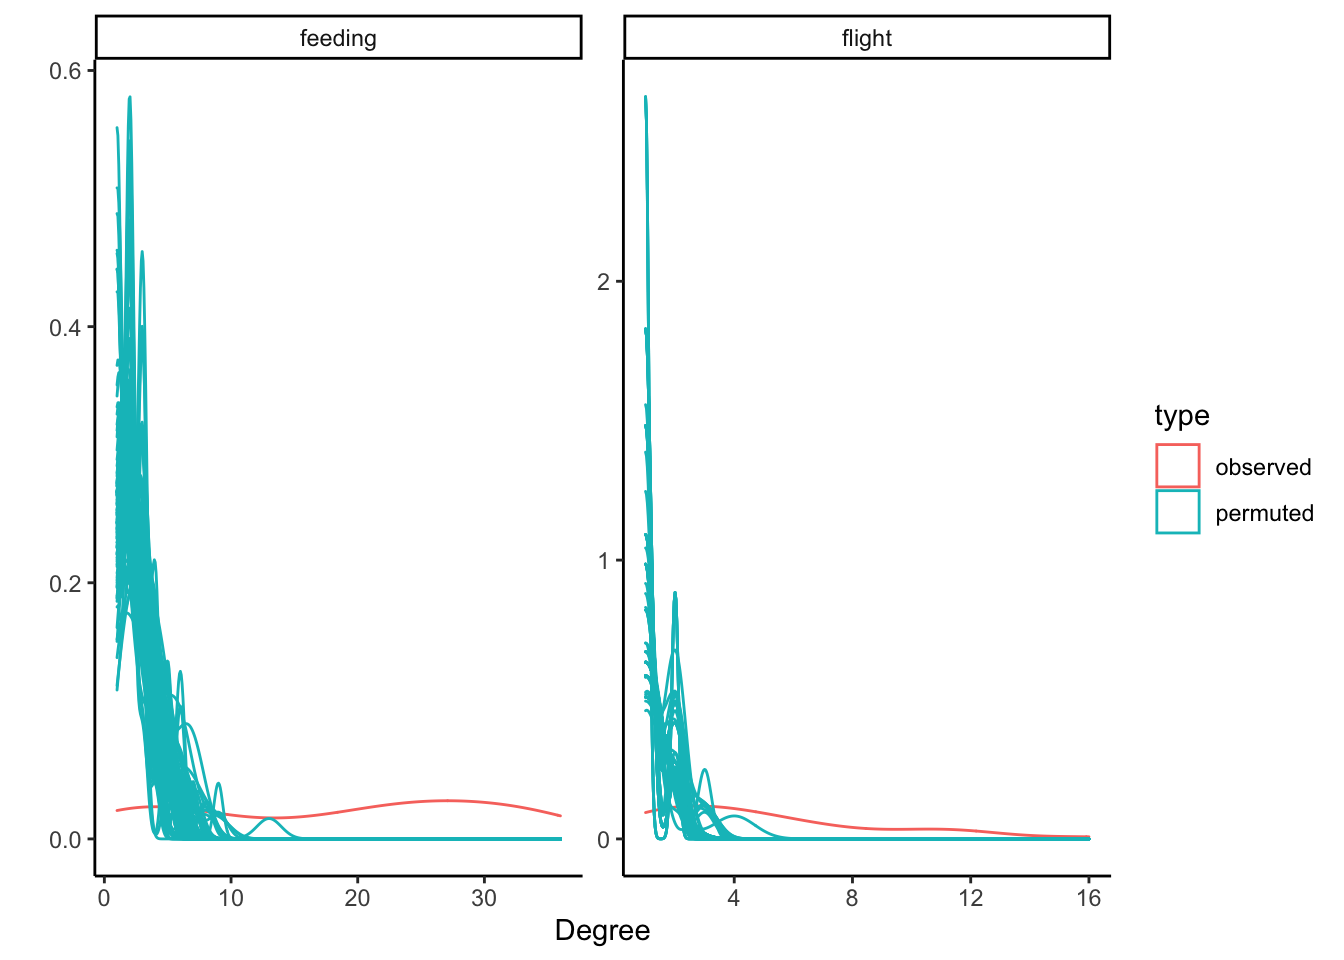
\includegraphics{arrivalAtCarcasses_files/figure-latex/unnamed-chunk-13-1.pdf}

Okay, now that I know how to plot points and I know when and where the
feeding events have occurred, time to plot points around each feeding
station, color-coded by individual, around the time of the feeding
events.

\begin{Shaded}
\begin{Highlighting}[]
\FunctionTok{head}\NormalTok{(feedEvents)}
\end{Highlighting}
\end{Shaded}

\begin{verbatim}
## Simple feature collection with 6 features and 10 fields
## Geometry type: POINT
## Dimension:     XY
## Bounding box:  xmin: 34.777 ymin: 30.8615 xmax: 35.3305 ymax: 31.3321
## Geodetic CRS:  WGS 84
##   feeding_date feeding_time                 area   feeding_station
## 1    8/30/2020  11:30:00 AM      SdeBoker_Hatira       Tzaror_trap
## 2     9/1/2020   2:15:00 PM Small_and_Big_crater Small_crater_view
## 3     9/4/2020  10:55:00 AM      SdeBoker_Hatira       Tzaror_trap
## 4     9/6/2020  11:10:00 AM  South_Judean_desert     Ben_Yair_view
## 5     9/7/2020   9:20:00 AM      SdeBoker_Hatira          Antenas 
## 6    9/12/2020  10:00:00 AM      SdeBoker_Hatira       Tzaror_trap
##           carcass_type weight_of_food no_of_carcasses            datetime
## 1 donkey, sheep, horse            350               3 2020-08-30 10:56:53
## 2          ibex, sheep            130               3 2020-09-01 13:16:41
## 3          sheep, calf            310               7 2020-09-04 09:55:39
## 4           sheep, cow            660               2 2020-09-06 10:13:52
## 5                  cow            600               1 2020-09-07 08:40:28
## 6          sheep, calf            300               6 2020-09-12 09:00:47
##       lat    long                geometry
## 1 30.8615 34.8136 POINT (34.8136 30.8615)
## 2 30.9490 35.1508  POINT (35.1508 30.949)
## 3 30.8615 34.8136 POINT (34.8136 30.8615)
## 4 31.3321 35.3305 POINT (35.3305 31.3321)
## 5 30.9349 34.7770  POINT (34.777 30.9349)
## 6 30.8615 34.8136 POINT (34.8136 30.8615)
\end{verbatim}

\begin{Shaded}
\begin{Highlighting}[]
\CommentTok{\# plot just the feeding events}
\NormalTok{feedEvents }\SpecialCharTok{\%\textgreater{}\%}
  \FunctionTok{ggplot}\NormalTok{(}\FunctionTok{aes}\NormalTok{(}\AttributeTok{x =}\NormalTok{ long, }\AttributeTok{y =}\NormalTok{ lat, }\AttributeTok{col =} \FunctionTok{as.numeric}\NormalTok{(datetime)))}\SpecialCharTok{+}
  \FunctionTok{geom\_point}\NormalTok{(}\AttributeTok{size =} \DecValTok{2}\NormalTok{)}\SpecialCharTok{+}
  \FunctionTok{scale\_color\_viridis\_c}\NormalTok{()}
\end{Highlighting}
\end{Shaded}

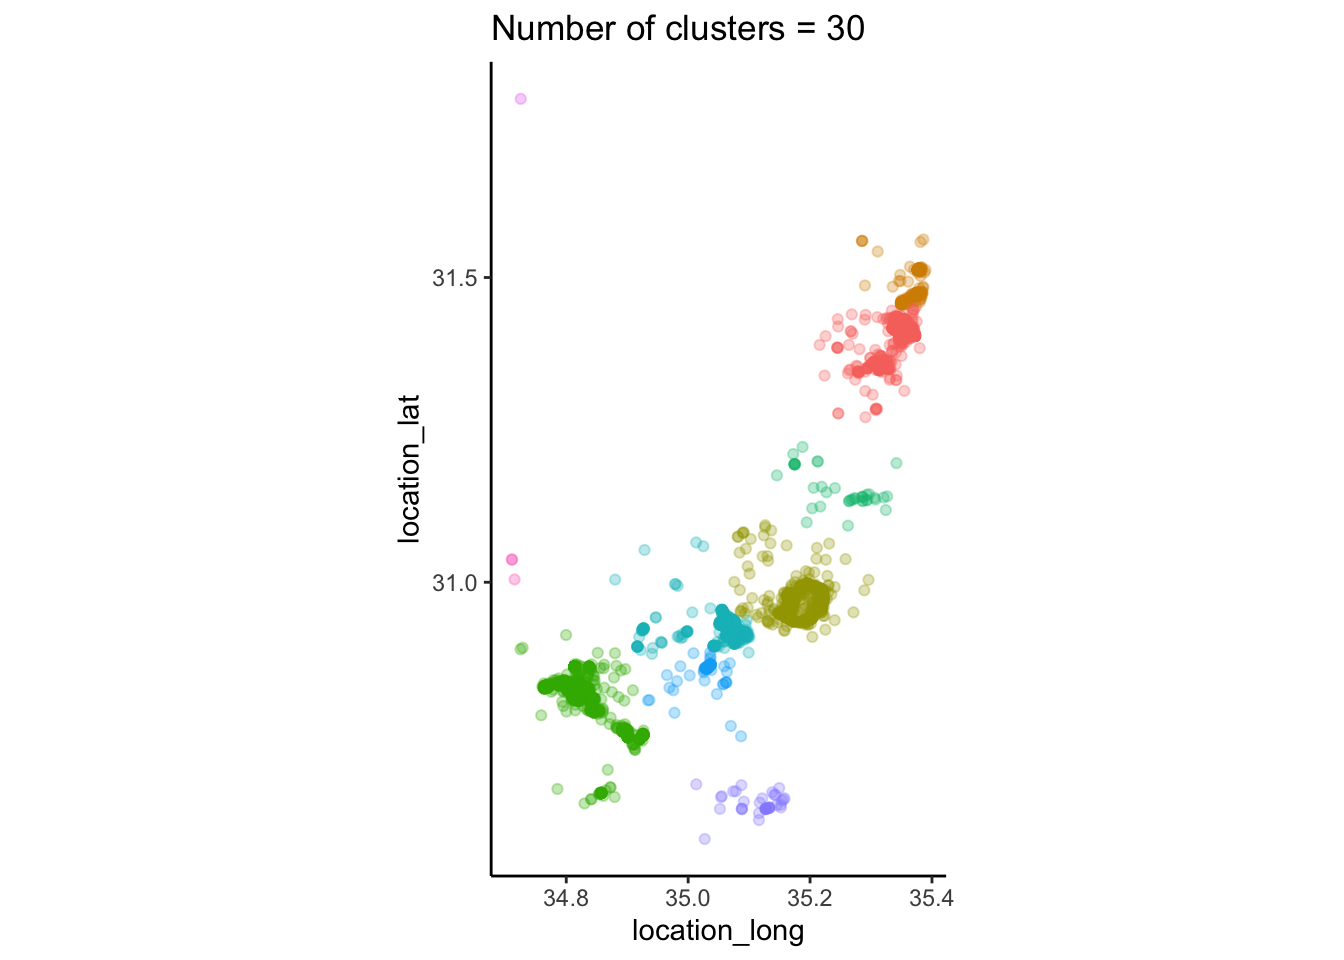
\includegraphics{arrivalAtCarcasses_files/figure-latex/unnamed-chunk-14-1.pdf}

\begin{Shaded}
\begin{Highlighting}[]
\CommentTok{\# Let\textquotesingle{}s pick the most recent feeding event to test with}
\NormalTok{event }\OtherTok{\textless{}{-}}\NormalTok{ feedEvents }\SpecialCharTok{\%\textgreater{}\%}
  \FunctionTok{slice}\NormalTok{(}\DecValTok{1}\NormalTok{)}

\CommentTok{\# In the supplementary material of Harel et al. 2016, it says that carcasses are usually discovered and consumed within "a few days," and that feeding by other scavengers also contributes to this. To be conservative, I\textquotesingle{}m going to examine a 4{-}day period after carcass deposition, regardless of when the vultures find the carcass.}
\CommentTok{\# Filter the data to just get the data 2 hours before up to 24*4 = 96 hours later than the feeding time.}
\NormalTok{maxTimeWords }\OtherTok{\textless{}{-}} \StringTok{"96 hours"}
\NormalTok{maxTime }\OtherTok{\textless{}{-}} \DecValTok{96}
\NormalTok{thisEvent }\OtherTok{\textless{}{-}}\NormalTok{ datMasked }\SpecialCharTok{\%\textgreater{}\%}
  \FunctionTok{filter}\NormalTok{(timestamp }\SpecialCharTok{\textgreater{}}\NormalTok{ event}\SpecialCharTok{$}\NormalTok{datetime[}\DecValTok{5}\NormalTok{] }\SpecialCharTok{{-}}\NormalTok{ lubridate}\SpecialCharTok{::}\FunctionTok{as.duration}\NormalTok{(}\StringTok{"2 hours"}\NormalTok{) }\SpecialCharTok{\&}\NormalTok{ timestamp }\SpecialCharTok{\textless{}}\NormalTok{ event}\SpecialCharTok{$}\NormalTok{datetime[}\DecValTok{5}\NormalTok{] }\SpecialCharTok{+}\NormalTok{ lubridate}\SpecialCharTok{::}\FunctionTok{as.duration}\NormalTok{(maxTimeWords))}
\CommentTok{\# I have not yet restricted this spatially.}

\NormalTok{bbox }\OtherTok{\textless{}{-}} \FunctionTok{bboxFromRad}\NormalTok{(}\AttributeTok{lon =}\NormalTok{ event}\SpecialCharTok{$}\NormalTok{long, }\AttributeTok{lat =}\NormalTok{ event}\SpecialCharTok{$}\NormalTok{lat, }\AttributeTok{kmDist =} \DecValTok{3}\NormalTok{)}
\NormalTok{map }\OtherTok{\textless{}{-}}\NormalTok{ ggmap}\SpecialCharTok{::}\FunctionTok{get\_stamenmap}\NormalTok{(}\AttributeTok{bbox =}\NormalTok{ bbox, }\AttributeTok{zoom =} \DecValTok{10}\NormalTok{, }\AttributeTok{maptype =} \StringTok{"terrain{-}background"}\NormalTok{)}
\end{Highlighting}
\end{Shaded}

\begin{verbatim}
## Source : http://tile.stamen.com/terrain-background/10/610/419.png
\end{verbatim}

\begin{verbatim}
## Source : http://tile.stamen.com/terrain-background/10/611/419.png
\end{verbatim}

\begin{Shaded}
\begin{Highlighting}[]
\FunctionTok{ggmap}\NormalTok{(map)}\SpecialCharTok{+}
  \FunctionTok{geom\_point}\NormalTok{(}\AttributeTok{data =}\NormalTok{ thisEvent, }\FunctionTok{aes}\NormalTok{(}\AttributeTok{x =}\NormalTok{ location\_long}\FloatTok{.1}\NormalTok{, }\AttributeTok{y =}\NormalTok{ location\_lat}\FloatTok{.1}\NormalTok{, }\AttributeTok{col =}\NormalTok{ trackId), }\AttributeTok{size =} \DecValTok{1}\NormalTok{)}\SpecialCharTok{+}
  \CommentTok{\#geom\_path(data = thisEvent, aes(x = location\_long.1, y = location\_lat.1, col = trackId), size = 0.5)+}
  \FunctionTok{geom\_point}\NormalTok{(}\AttributeTok{data =}\NormalTok{ event, }\FunctionTok{aes}\NormalTok{(}\AttributeTok{x =}\NormalTok{ long, }\AttributeTok{y =}\NormalTok{ lat), }\AttributeTok{col =} \StringTok{"black"}\NormalTok{, }\AttributeTok{size =} \DecValTok{3}\NormalTok{)}\SpecialCharTok{+}
  \FunctionTok{scale\_color\_viridis\_d}\NormalTok{()}\SpecialCharTok{+}
  \FunctionTok{theme}\NormalTok{(}\AttributeTok{legend.position =} \StringTok{"none"}\NormalTok{)}
\end{Highlighting}
\end{Shaded}

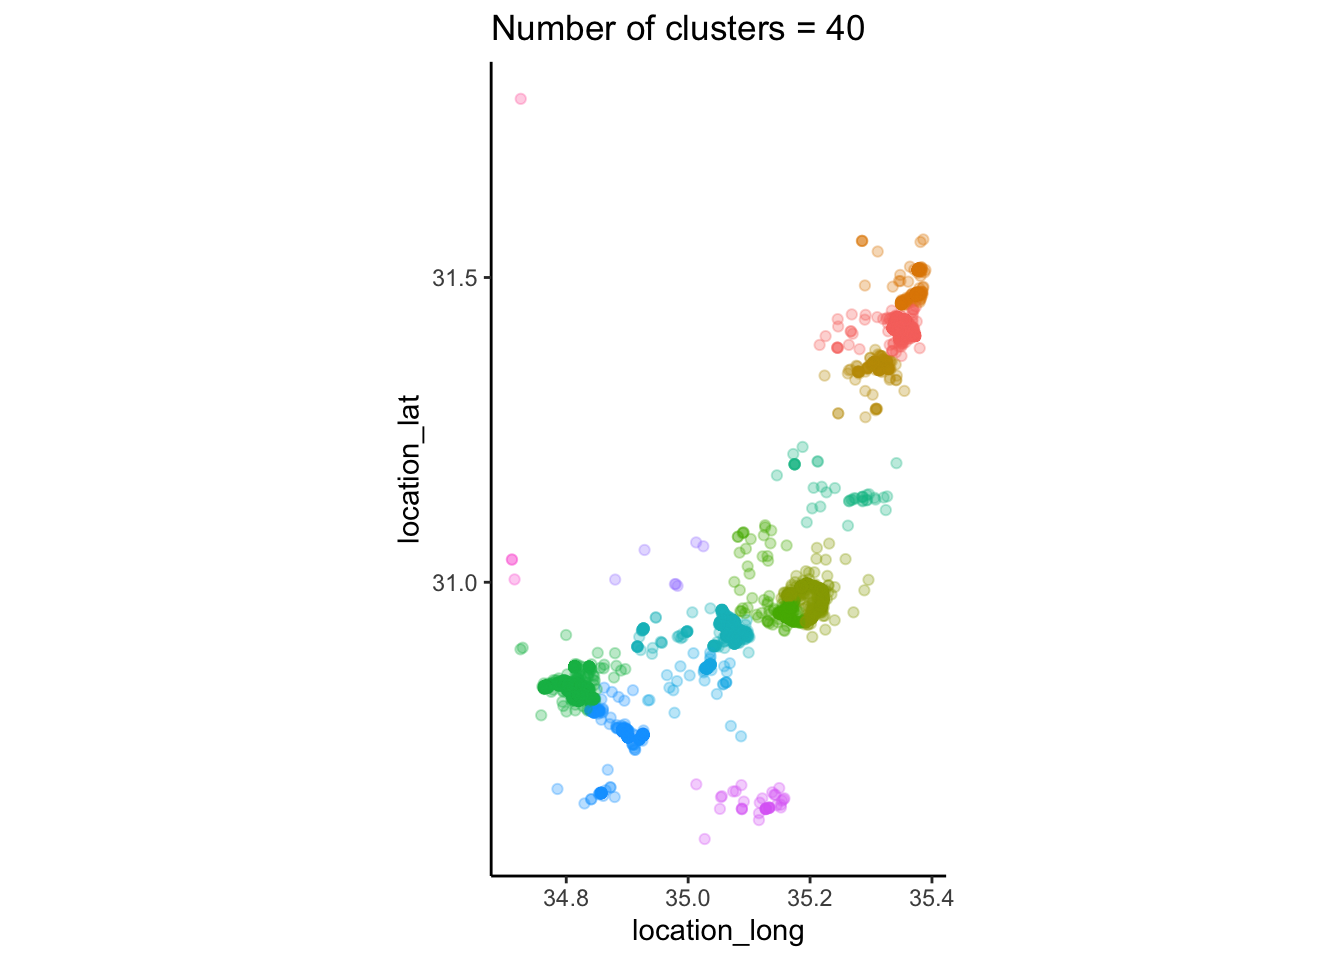
\includegraphics{arrivalAtCarcasses_files/figure-latex/unnamed-chunk-14-2.pdf}

\hypertarget{distance-from-carcass-vs.-time}{%
\subsubsection{Distance from carcass
vs.~time}\label{distance-from-carcass-vs.-time}}

In the supplementary material of Harel et al.~2016, it says that
carcasses are usually discovered and consumed within ``a few days,'' and
that feeding by other scavengers also contributes to this. To be
conservative, I'm going to examine a 4-day period after carcass
deposition, regardless of when the vultures find the carcass. So that's
96 hours.

I was going to try to animate this, but instead I'm just going to
calculate distance over time and plot it. Duh.

Do this for all feeding events.

\begin{Shaded}
\begin{Highlighting}[]
\CommentTok{\# Make a list of the datasets for each feeding event, ranging from 2 hours before carcass placement through 200 hours after carcass placement. For each point in the dataset, calculate the distance from the carcass.}
\NormalTok{eventsList }\OtherTok{\textless{}{-}}\NormalTok{ feedEvents }\SpecialCharTok{\%\textgreater{}\%}
  \FunctionTok{group\_by}\NormalTok{(datetime) }\SpecialCharTok{\%\textgreater{}\%}
  \FunctionTok{group\_split}\NormalTok{(}\AttributeTok{.keep =}\NormalTok{ T)}
\FunctionTok{length}\NormalTok{(eventsList)}

\NormalTok{eventsDat }\OtherTok{\textless{}{-}} \FunctionTok{lapply}\NormalTok{(eventsList, }\ControlFlowTok{function}\NormalTok{(x)\{}
\NormalTok{  dat }\OtherTok{\textless{}{-}}\NormalTok{ datMasked }\SpecialCharTok{\%\textgreater{}\%}
    \FunctionTok{filter}\NormalTok{(timestamp }\SpecialCharTok{\textgreater{}}\NormalTok{ x}\SpecialCharTok{$}\NormalTok{datetime[}\DecValTok{1}\NormalTok{]}\SpecialCharTok{{-}}\NormalTok{lubridate}\SpecialCharTok{::}\FunctionTok{as.duration}\NormalTok{(}\StringTok{"2 hours"}\NormalTok{) }\SpecialCharTok{\&}\NormalTok{ timestamp }\SpecialCharTok{\textless{}}\NormalTok{ x}\SpecialCharTok{$}\NormalTok{datetime[}\DecValTok{1}\NormalTok{] }\SpecialCharTok{+}\NormalTok{ lubridate}\SpecialCharTok{::}\FunctionTok{as.duration}\NormalTok{(maxTimeWords)) }\SpecialCharTok{\%\textgreater{}\%}
    \FunctionTok{mutate}\NormalTok{(}\AttributeTok{timeSinceCarcassPlaced =}\NormalTok{ timestamp }\SpecialCharTok{{-}}\NormalTok{ x}\SpecialCharTok{$}\NormalTok{datetime[}\DecValTok{1}\NormalTok{])}
\NormalTok{\})}

\NormalTok{eventsDat }\OtherTok{\textless{}{-}} \FunctionTok{map2}\NormalTok{(}\AttributeTok{.x =}\NormalTok{ eventsDat, }\AttributeTok{.y =}\NormalTok{ eventsList, }\AttributeTok{.f =} \ControlFlowTok{function}\NormalTok{(.x, .y)\{}
\NormalTok{  .x }\OtherTok{\textless{}{-}}\NormalTok{ .x }\SpecialCharTok{\%\textgreater{}\%}
    \FunctionTok{mutate}\NormalTok{(}\AttributeTok{distanceFromCarcass =} \FunctionTok{as.numeric}\NormalTok{(sf}\SpecialCharTok{::}\FunctionTok{st\_distance}\NormalTok{(., .y))}\SpecialCharTok{/}\DecValTok{1000}\NormalTok{)}
\NormalTok{\})}

\CommentTok{\# download elevation rasters for points within 3km of each feeding event}
\NormalTok{eventsDat3km }\OtherTok{\textless{}{-}} \FunctionTok{lapply}\NormalTok{(eventsDat, }\ControlFlowTok{function}\NormalTok{(x)\{}
\NormalTok{  x }\SpecialCharTok{\%\textgreater{}\%}
    \FunctionTok{filter}\NormalTok{(distanceFromCarcass }\SpecialCharTok{\textless{}} \DecValTok{3}\NormalTok{)}
\NormalTok{\})}

\NormalTok{elevRasters }\OtherTok{\textless{}{-}} \FunctionTok{lapply}\NormalTok{(eventsDat3km, }\ControlFlowTok{function}\NormalTok{(x)\{}
  \ControlFlowTok{if}\NormalTok{(}\FunctionTok{nrow}\NormalTok{(x) }\SpecialCharTok{==} \DecValTok{0}\NormalTok{)\{}
    \FunctionTok{return}\NormalTok{(}\ConstantTok{NULL}\NormalTok{)}
\NormalTok{  \}}\ControlFlowTok{else}\NormalTok{\{}
\NormalTok{    elev }\OtherTok{\textless{}{-}}\NormalTok{ elevatr}\SpecialCharTok{::}\FunctionTok{get\_elev\_raster}\NormalTok{(x, }\AttributeTok{z =} \DecValTok{12}\NormalTok{)}
    \FunctionTok{return}\NormalTok{(elev)}
\NormalTok{  \}}
\NormalTok{\})}
\end{Highlighting}
\end{Shaded}

\begin{verbatim}
## Mosaicing & Projecting
\end{verbatim}

\begin{verbatim}
## Note: Elevation units are in meters.
\end{verbatim}

\begin{verbatim}
## Mosaicing & Projecting
\end{verbatim}

\begin{verbatim}
## Note: Elevation units are in meters.
\end{verbatim}

\begin{verbatim}
## Mosaicing & Projecting
\end{verbatim}

\begin{verbatim}
## Note: Elevation units are in meters.
\end{verbatim}

\begin{verbatim}
## Mosaicing & Projecting
\end{verbatim}

\begin{verbatim}
## Note: Elevation units are in meters.
\end{verbatim}

\begin{verbatim}
## Mosaicing & Projecting
\end{verbatim}

\begin{verbatim}
## Note: Elevation units are in meters.
\end{verbatim}

\begin{verbatim}
## Mosaicing & Projecting
\end{verbatim}

\begin{verbatim}
## Note: Elevation units are in meters.
\end{verbatim}

\begin{verbatim}
## Mosaicing & Projecting
\end{verbatim}

\begin{verbatim}
## Note: Elevation units are in meters.
\end{verbatim}

\begin{verbatim}
## Mosaicing & Projecting
\end{verbatim}

\begin{verbatim}
## Note: Elevation units are in meters.
\end{verbatim}

\begin{verbatim}
## Mosaicing & Projecting
\end{verbatim}

\begin{verbatim}
## Note: Elevation units are in meters.
\end{verbatim}

\begin{verbatim}
## Mosaicing & Projecting
\end{verbatim}

\begin{verbatim}
## Note: Elevation units are in meters.
\end{verbatim}

\begin{verbatim}
## Mosaicing & Projecting
\end{verbatim}

\begin{verbatim}
## Note: Elevation units are in meters.
\end{verbatim}

\begin{verbatim}
## Mosaicing & Projecting
\end{verbatim}

\begin{verbatim}
## Note: Elevation units are in meters.
\end{verbatim}

\begin{verbatim}
## Mosaicing & Projecting
\end{verbatim}

\begin{verbatim}
## Note: Elevation units are in meters.
\end{verbatim}

\begin{verbatim}
## Mosaicing & Projecting
\end{verbatim}

\begin{verbatim}
## Note: Elevation units are in meters.
\end{verbatim}

\begin{verbatim}
## Mosaicing & Projecting
\end{verbatim}

\begin{verbatim}
## Note: Elevation units are in meters.
\end{verbatim}

\begin{verbatim}
## Mosaicing & Projecting
\end{verbatim}

\begin{verbatim}
## Note: Elevation units are in meters.
\end{verbatim}

\begin{verbatim}
## Mosaicing & Projecting
\end{verbatim}

\begin{verbatim}
## Note: Elevation units are in meters.
\end{verbatim}

\begin{verbatim}
## Mosaicing & Projecting
\end{verbatim}

\begin{verbatim}
## Note: Elevation units are in meters.
\end{verbatim}

\begin{verbatim}
## Mosaicing & Projecting
\end{verbatim}

\begin{verbatim}
## Note: Elevation units are in meters.
\end{verbatim}

\begin{verbatim}
## Mosaicing & Projecting
\end{verbatim}

\begin{verbatim}
## Note: Elevation units are in meters.
\end{verbatim}

\begin{verbatim}
## Mosaicing & Projecting
\end{verbatim}

\begin{verbatim}
## Note: Elevation units are in meters.
\end{verbatim}

\begin{verbatim}
## Mosaicing & Projecting
\end{verbatim}

\begin{verbatim}
## Note: Elevation units are in meters.
\end{verbatim}

\begin{verbatim}
## Mosaicing & Projecting
\end{verbatim}

\begin{verbatim}
## Note: Elevation units are in meters.
\end{verbatim}

\begin{verbatim}
## Mosaicing & Projecting
\end{verbatim}

\begin{verbatim}
## Note: Elevation units are in meters.
\end{verbatim}

\begin{verbatim}
## Mosaicing & Projecting
\end{verbatim}

\begin{verbatim}
## Note: Elevation units are in meters.
\end{verbatim}

\begin{verbatim}
## Mosaicing & Projecting
\end{verbatim}

\begin{verbatim}
## Note: Elevation units are in meters.
\end{verbatim}

\begin{verbatim}
## Mosaicing & Projecting
\end{verbatim}

\begin{verbatim}
## Note: Elevation units are in meters.
\end{verbatim}

\begin{verbatim}
## Mosaicing & Projecting
\end{verbatim}

\begin{verbatim}
## Note: Elevation units are in meters.
\end{verbatim}

\begin{verbatim}
## Mosaicing & Projecting
\end{verbatim}

\begin{verbatim}
## Note: Elevation units are in meters.
\end{verbatim}

\begin{verbatim}
## Mosaicing & Projecting
\end{verbatim}

\begin{verbatim}
## Note: Elevation units are in meters.
\end{verbatim}

\begin{verbatim}
## Mosaicing & Projecting
\end{verbatim}

\begin{verbatim}
## Note: Elevation units are in meters.
\end{verbatim}

\begin{verbatim}
## Mosaicing & Projecting
\end{verbatim}

\begin{verbatim}
## Note: Elevation units are in meters.
\end{verbatim}

\begin{verbatim}
## Mosaicing & Projecting
\end{verbatim}

\begin{verbatim}
## Note: Elevation units are in meters.
\end{verbatim}

\begin{verbatim}
## Mosaicing & Projecting
\end{verbatim}

\begin{verbatim}
## Note: Elevation units are in meters.
\end{verbatim}

\begin{verbatim}
## Mosaicing & Projecting
\end{verbatim}

\begin{verbatim}
## Note: Elevation units are in meters.
\end{verbatim}

\begin{verbatim}
## Mosaicing & Projecting
\end{verbatim}

\begin{verbatim}
## Note: Elevation units are in meters.
\end{verbatim}

\begin{verbatim}
## Mosaicing & Projecting
\end{verbatim}

\begin{verbatim}
## Note: Elevation units are in meters.
\end{verbatim}

\begin{verbatim}
## Mosaicing & Projecting
\end{verbatim}

\begin{verbatim}
## Note: Elevation units are in meters.
\end{verbatim}

\begin{verbatim}
## Mosaicing & Projecting
\end{verbatim}

\begin{verbatim}
## Note: Elevation units are in meters.
\end{verbatim}

\begin{verbatim}
## Mosaicing & Projecting
\end{verbatim}

\begin{verbatim}
## Note: Elevation units are in meters.
\end{verbatim}

\begin{verbatim}
## Mosaicing & Projecting
\end{verbatim}

\begin{verbatim}
## Note: Elevation units are in meters.
\end{verbatim}

\begin{verbatim}
## Mosaicing & Projecting
\end{verbatim}

\begin{verbatim}
## Note: Elevation units are in meters.
\end{verbatim}

\begin{Shaded}
\begin{Highlighting}[]
\CommentTok{\# add elevation information to data frames, but only for the points within 3km of the feeding site.}
\NormalTok{eventsDat }\OtherTok{\textless{}{-}} \FunctionTok{map2}\NormalTok{(}\AttributeTok{.x =}\NormalTok{ eventsDat, }\AttributeTok{.y =}\NormalTok{ elevRasters, }\AttributeTok{.f =} \ControlFlowTok{function}\NormalTok{(.x, .y)\{}
  \ControlFlowTok{if}\NormalTok{(}\FunctionTok{is.null}\NormalTok{(.y))\{}
\NormalTok{    .x }\OtherTok{\textless{}{-}}\NormalTok{ .x }\SpecialCharTok{\%\textgreater{}\%}
      \FunctionTok{mutate}\NormalTok{(}\AttributeTok{groundElev =} \ConstantTok{NA}\NormalTok{,}
             \AttributeTok{height\_above\_ground =} \ConstantTok{NA}\NormalTok{)}
\NormalTok{  \}}\ControlFlowTok{else}\NormalTok{\{}
\NormalTok{    .x }\OtherTok{\textless{}{-}}\NormalTok{ .x }\SpecialCharTok{\%\textgreater{}\%}
      \FunctionTok{mutate}\NormalTok{(}\AttributeTok{groundElev =}\NormalTok{ raster}\SpecialCharTok{::}\FunctionTok{extract}\NormalTok{(.y, .x),}
             \AttributeTok{height\_above\_ground =}\NormalTok{ height\_above\_msl }\SpecialCharTok{{-}}\NormalTok{ groundElev) }\SpecialCharTok{\%\textgreater{}\%}
      \FunctionTok{mutate}\NormalTok{(}\AttributeTok{height\_above\_ground =} \FunctionTok{case\_when}\NormalTok{(height\_above\_ground }\SpecialCharTok{\textless{}} \DecValTok{0} \SpecialCharTok{\textasciitilde{}} \DecValTok{0}\NormalTok{,}
                                             \ConstantTok{TRUE} \SpecialCharTok{\textasciitilde{}}\NormalTok{ height\_above\_ground))}
\NormalTok{  \}}
\NormalTok{\})}

\CommentTok{\# Now we can use this to make the same plot for each feeding event, limiting it to a certain radius}
\NormalTok{plots }\OtherTok{\textless{}{-}} \FunctionTok{map2}\NormalTok{(}\AttributeTok{.x =}\NormalTok{ eventsDat, }\AttributeTok{.y =}\NormalTok{ eventsList, }\AttributeTok{.f =} \ControlFlowTok{function}\NormalTok{(.x, .y)\{}
  \CommentTok{\# min \textless{}{-} min(.x$timestamp[.x$distanceFromCarcass \textless{}= 20])}
  \CommentTok{\# max \textless{}{-} max(.x$timestamp[.x$distanceFromCarcass \textless{}= 20])}
\NormalTok{  p }\OtherTok{\textless{}{-}}\NormalTok{ .x }\SpecialCharTok{\%\textgreater{}\%}
    \FunctionTok{ggplot}\NormalTok{()}\SpecialCharTok{+}
    \FunctionTok{geom\_point}\NormalTok{(}\FunctionTok{aes}\NormalTok{(}\AttributeTok{x =}\NormalTok{ timestamp, }\AttributeTok{y =}\NormalTok{ distanceFromCarcass, }\AttributeTok{col =}\NormalTok{ trackId))}\SpecialCharTok{+}
    \FunctionTok{geom\_line}\NormalTok{(}\FunctionTok{aes}\NormalTok{(}\AttributeTok{x =}\NormalTok{ timestamp, }\AttributeTok{y =}\NormalTok{ distanceFromCarcass, }\AttributeTok{col =}\NormalTok{ trackId))}\SpecialCharTok{+}
    \FunctionTok{geom\_vline}\NormalTok{(}\AttributeTok{data =}\NormalTok{ .y, }\FunctionTok{aes}\NormalTok{(}\AttributeTok{xintercept =}\NormalTok{ .y}\SpecialCharTok{$}\NormalTok{datetime[}\DecValTok{1}\NormalTok{]))}\SpecialCharTok{+}
    \FunctionTok{theme\_minimal}\NormalTok{()}\SpecialCharTok{+}
    \FunctionTok{ylim}\NormalTok{(}\DecValTok{0}\NormalTok{, }\DecValTok{20}\NormalTok{)}
\NormalTok{\})}
\FunctionTok{suppressWarnings}\NormalTok{(}\FunctionTok{print}\NormalTok{(plots))}
\end{Highlighting}
\end{Shaded}

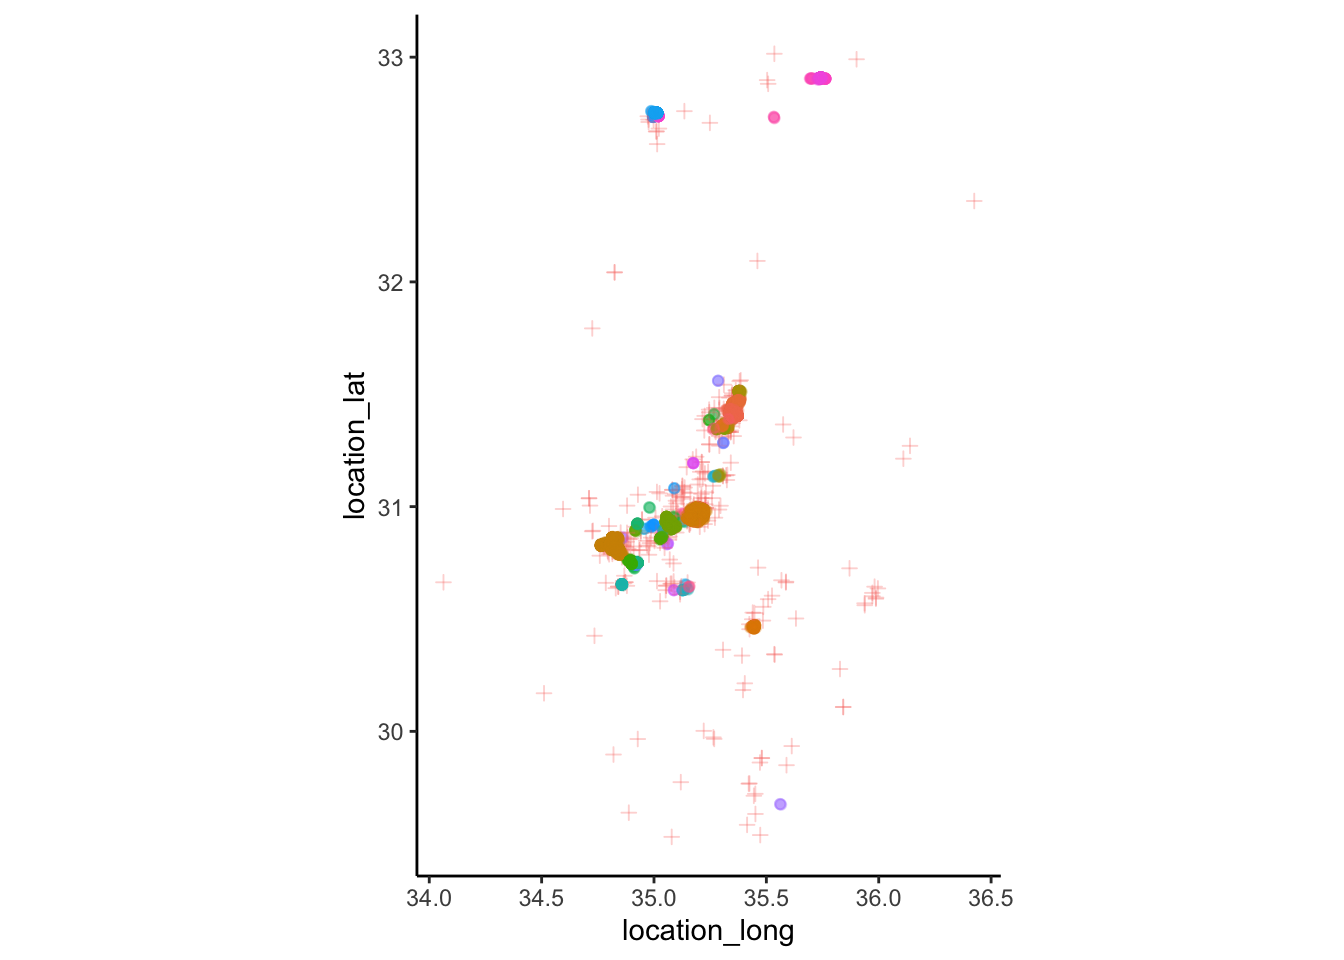
\includegraphics{arrivalAtCarcasses_files/figure-latex/unnamed-chunk-15-1.pdf}
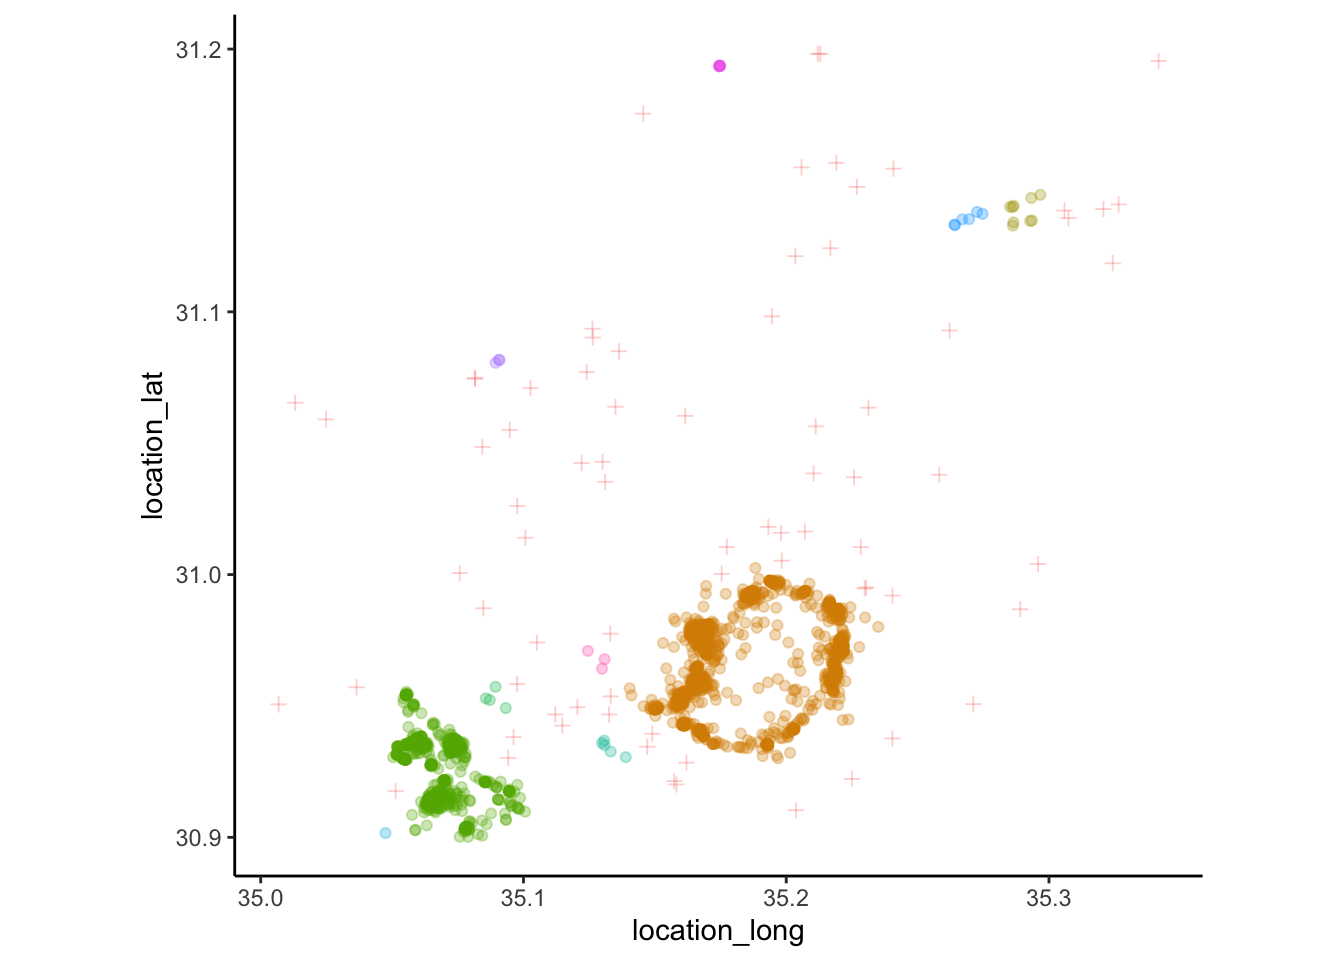
\includegraphics{arrivalAtCarcasses_files/figure-latex/unnamed-chunk-15-2.pdf}
\includegraphics{arrivalAtCarcasses_files/figure-latex/unnamed-chunk-15-3.pdf}
\includegraphics{arrivalAtCarcasses_files/figure-latex/unnamed-chunk-15-4.pdf}
\includegraphics{arrivalAtCarcasses_files/figure-latex/unnamed-chunk-15-5.pdf}
\includegraphics{arrivalAtCarcasses_files/figure-latex/unnamed-chunk-15-6.pdf}
\includegraphics{arrivalAtCarcasses_files/figure-latex/unnamed-chunk-15-7.pdf}
\includegraphics{arrivalAtCarcasses_files/figure-latex/unnamed-chunk-15-8.pdf}
\includegraphics{arrivalAtCarcasses_files/figure-latex/unnamed-chunk-15-9.pdf}
\includegraphics{arrivalAtCarcasses_files/figure-latex/unnamed-chunk-15-10.pdf}
\includegraphics{arrivalAtCarcasses_files/figure-latex/unnamed-chunk-15-11.pdf}
\includegraphics{arrivalAtCarcasses_files/figure-latex/unnamed-chunk-15-12.pdf}
\includegraphics{arrivalAtCarcasses_files/figure-latex/unnamed-chunk-15-13.pdf}
\includegraphics{arrivalAtCarcasses_files/figure-latex/unnamed-chunk-15-14.pdf}
\includegraphics{arrivalAtCarcasses_files/figure-latex/unnamed-chunk-15-15.pdf}
\includegraphics{arrivalAtCarcasses_files/figure-latex/unnamed-chunk-15-16.pdf}
\includegraphics{arrivalAtCarcasses_files/figure-latex/unnamed-chunk-15-17.pdf}
\includegraphics{arrivalAtCarcasses_files/figure-latex/unnamed-chunk-15-18.pdf}
\includegraphics{arrivalAtCarcasses_files/figure-latex/unnamed-chunk-15-19.pdf}
\includegraphics{arrivalAtCarcasses_files/figure-latex/unnamed-chunk-15-20.pdf}
\includegraphics{arrivalAtCarcasses_files/figure-latex/unnamed-chunk-15-21.pdf}
\includegraphics{arrivalAtCarcasses_files/figure-latex/unnamed-chunk-15-22.pdf}
\includegraphics{arrivalAtCarcasses_files/figure-latex/unnamed-chunk-15-23.pdf}
\includegraphics{arrivalAtCarcasses_files/figure-latex/unnamed-chunk-15-24.pdf}
\includegraphics{arrivalAtCarcasses_files/figure-latex/unnamed-chunk-15-25.pdf}
\includegraphics{arrivalAtCarcasses_files/figure-latex/unnamed-chunk-15-26.pdf}
\includegraphics{arrivalAtCarcasses_files/figure-latex/unnamed-chunk-15-27.pdf}
\includegraphics{arrivalAtCarcasses_files/figure-latex/unnamed-chunk-15-28.pdf}
\includegraphics{arrivalAtCarcasses_files/figure-latex/unnamed-chunk-15-29.pdf}
\includegraphics{arrivalAtCarcasses_files/figure-latex/unnamed-chunk-15-30.pdf}
\includegraphics{arrivalAtCarcasses_files/figure-latex/unnamed-chunk-15-31.pdf}
\includegraphics{arrivalAtCarcasses_files/figure-latex/unnamed-chunk-15-32.pdf}
\includegraphics{arrivalAtCarcasses_files/figure-latex/unnamed-chunk-15-33.pdf}
\includegraphics{arrivalAtCarcasses_files/figure-latex/unnamed-chunk-15-34.pdf}
\includegraphics{arrivalAtCarcasses_files/figure-latex/unnamed-chunk-15-35.pdf}
\includegraphics{arrivalAtCarcasses_files/figure-latex/unnamed-chunk-15-36.pdf}
\includegraphics{arrivalAtCarcasses_files/figure-latex/unnamed-chunk-15-37.pdf}
\includegraphics{arrivalAtCarcasses_files/figure-latex/unnamed-chunk-15-38.pdf}
\includegraphics{arrivalAtCarcasses_files/figure-latex/unnamed-chunk-15-39.pdf}
\includegraphics{arrivalAtCarcasses_files/figure-latex/unnamed-chunk-15-40.pdf}
\includegraphics{arrivalAtCarcasses_files/figure-latex/unnamed-chunk-15-41.pdf}
\includegraphics{arrivalAtCarcasses_files/figure-latex/unnamed-chunk-15-42.pdf}
\includegraphics{arrivalAtCarcasses_files/figure-latex/unnamed-chunk-15-43.pdf}
\includegraphics{arrivalAtCarcasses_files/figure-latex/unnamed-chunk-15-44.pdf}
\includegraphics{arrivalAtCarcasses_files/figure-latex/unnamed-chunk-15-45.pdf}
\includegraphics{arrivalAtCarcasses_files/figure-latex/unnamed-chunk-15-46.pdf}
\includegraphics{arrivalAtCarcasses_files/figure-latex/unnamed-chunk-15-47.pdf}
\includegraphics{arrivalAtCarcasses_files/figure-latex/unnamed-chunk-15-48.pdf}
\includegraphics{arrivalAtCarcasses_files/figure-latex/unnamed-chunk-15-49.pdf}
\includegraphics{arrivalAtCarcasses_files/figure-latex/unnamed-chunk-15-50.pdf}
\includegraphics{arrivalAtCarcasses_files/figure-latex/unnamed-chunk-15-51.pdf}
\includegraphics{arrivalAtCarcasses_files/figure-latex/unnamed-chunk-15-52.pdf}
\includegraphics{arrivalAtCarcasses_files/figure-latex/unnamed-chunk-15-53.pdf}
\includegraphics{arrivalAtCarcasses_files/figure-latex/unnamed-chunk-15-54.pdf}
\includegraphics{arrivalAtCarcasses_files/figure-latex/unnamed-chunk-15-55.pdf}

\hypertarget{detections-and-arrivals}{%
\subsubsection{Detections and arrivals}\label{detections-and-arrivals}}

\begin{enumerate}
\def\labelenumi{\arabic{enumi}.}
\tightlist
\item
  Define ``detection'' as a vulture passing within 1km of the site,
  regardless of speed or altitude.
\item
  Define ``arrival'' as being within 0.25km with a ground speed
  \textless{} 5m/s and an elevation \textless{} 10m Calculate detections
  and arrivals for each bird at each carcass.
\end{enumerate}

\begin{Shaded}
\begin{Highlighting}[]
\NormalTok{eventsDat }\OtherTok{\textless{}{-}} \FunctionTok{lapply}\NormalTok{(eventsDat, }\ControlFlowTok{function}\NormalTok{(x)\{}
\NormalTok{  x }\OtherTok{\textless{}{-}}\NormalTok{ x }\SpecialCharTok{\%\textgreater{}\%}
    \FunctionTok{mutate}\NormalTok{(}\AttributeTok{detection =} \FunctionTok{case\_when}\NormalTok{(distanceFromCarcass }\SpecialCharTok{\textless{}} \DecValTok{1} \SpecialCharTok{\&} 
\NormalTok{                                   timeSinceCarcassPlaced }\SpecialCharTok{\textgreater{}} \DecValTok{0}  \SpecialCharTok{\textasciitilde{}} \ConstantTok{TRUE}\NormalTok{,}
                                 \ConstantTok{TRUE} \SpecialCharTok{\textasciitilde{}} \ConstantTok{FALSE}\NormalTok{),}
           \AttributeTok{visit =} \FunctionTok{case\_when}\NormalTok{(distanceFromCarcass }\SpecialCharTok{\textless{}} \FloatTok{0.25} \SpecialCharTok{\&}\NormalTok{ ground\_speed }\SpecialCharTok{\textless{}} \DecValTok{5} \SpecialCharTok{\&} 
                               \SpecialCharTok{!}\FunctionTok{is.na}\NormalTok{(height\_above\_ground) }\SpecialCharTok{\&}\NormalTok{ height\_above\_ground }\SpecialCharTok{\textless{}} \DecValTok{10} \SpecialCharTok{\&}
\NormalTok{                               timeSinceCarcassPlaced }\SpecialCharTok{\textgreater{}} \DecValTok{0} \SpecialCharTok{\textasciitilde{}} 
                               \ConstantTok{TRUE}\NormalTok{,}
                             \ConstantTok{TRUE} \SpecialCharTok{\textasciitilde{}} \ConstantTok{FALSE}\NormalTok{))}
\NormalTok{\})}
\end{Highlighting}
\end{Shaded}

\hypertarget{latency}{%
\subsubsection{Latency}\label{latency}}

\begin{Shaded}
\begin{Highlighting}[]
\NormalTok{allCarcasses }\OtherTok{\textless{}{-}}\NormalTok{ data.table}\SpecialCharTok{::}\FunctionTok{rbindlist}\NormalTok{(eventsDat, }\AttributeTok{idcol =} \StringTok{"eventID"}\NormalTok{) }\SpecialCharTok{\%\textgreater{}\%}
  \FunctionTok{as.data.frame}\NormalTok{() }\SpecialCharTok{\%\textgreater{}\%}
\NormalTok{  dplyr}\SpecialCharTok{::}\FunctionTok{select}\NormalTok{(eventID, ground\_speed, height\_above\_msl, location\_lat, location\_long, timestamp, dateOnly, trackId, geometry, timeSinceCarcassPlaced, distanceFromCarcass, groundElev, height\_above\_ground, detection, visit)}
\end{Highlighting}
\end{Shaded}

\hypertarget{time-to-first-detection}{%
\paragraph{Time to first detection}\label{time-to-first-detection}}

Let's assume that all carcasses will be detected within 10 days = 240
hours = 14400 minutes. So we'll filter the data down to that.

\begin{Shaded}
\begin{Highlighting}[]
\NormalTok{firstDetections }\OtherTok{\textless{}{-}}\NormalTok{ allCarcasses }\SpecialCharTok{\%\textgreater{}\%}
  \FunctionTok{filter}\NormalTok{(timeSinceCarcassPlaced }\SpecialCharTok{\textgreater{}} \DecValTok{0} \SpecialCharTok{\&}\NormalTok{ timeSinceCarcassPlaced }\SpecialCharTok{\textless{}}\NormalTok{ maxTime}\SpecialCharTok{*}\DecValTok{60}\NormalTok{, detection }\SpecialCharTok{==} \ConstantTok{TRUE}\NormalTok{) }\SpecialCharTok{\%\textgreater{}\%}
  \FunctionTok{group\_by}\NormalTok{(eventID) }\SpecialCharTok{\%\textgreater{}\%}
  \FunctionTok{arrange}\NormalTok{(timestamp, }\AttributeTok{.by\_group =} \ConstantTok{TRUE}\NormalTok{) }\SpecialCharTok{\%\textgreater{}\%}
  \FunctionTok{slice}\NormalTok{(}\DecValTok{1}\NormalTok{)}
\FunctionTok{glimpse}\NormalTok{(firstDetections)}
\end{Highlighting}
\end{Shaded}

\begin{verbatim}
## Rows: 26
## Columns: 15
## Groups: eventID [26]
## $ eventID                <int> 5, 6, 7, 8, 9, 11, 12, 13, 15, 16, 17, 18, 20, ~
## $ ground_speed           <dbl> 16.1111111, 4.1666667, 9.4444444, 0.0000000, 8.~
## $ height_above_msl       <dbl> 673, 769, 699, 506, 1451, 865, 797, 488, 387, 1~
## $ location_lat           <dbl> 30.93593, 30.86246, 30.89881, 30.86148, 30.6513~
## $ location_long          <dbl> 34.78006, 34.80872, 35.04202, 34.81364, 34.8489~
## $ timestamp              <dttm> 2020-09-08 07:43:08, 2020-09-12 09:02:30, 2020~
## $ dateOnly               <date> 2020-09-08, 2020-09-12, 2020-09-17, 2020-09-21~
## $ trackId                <chr> "J11w", "A03w", "J18w", "J16w", "J35w", "T99b",~
## $ geometry               <POINT [°]> POINT (34.78006 30.93593), POINT (34.8087~
## $ timeSinceCarcassPlaced <drtn> 1382.666667 mins, 103.000000 mins, 660.000000 ~
## $ distanceFromCarcass    <dbl> 0.313932528, 0.477437719, 0.401299332, 0.004350~
## $ groundElev             <dbl> 545, 485, 393, 497, 748, 302, 98, 461, 392, 354~
## $ height_above_ground    <dbl> 128, 284, 306, 9, 703, 563, 699, 27, 0, 1032, 1~
## $ detection              <lgl> TRUE, TRUE, TRUE, TRUE, TRUE, TRUE, TRUE, TRUE,~
## $ visit                  <lgl> FALSE, FALSE, FALSE, TRUE, FALSE, FALSE, FALSE,~
\end{verbatim}

\begin{Shaded}
\begin{Highlighting}[]
\NormalTok{firstDetections }\SpecialCharTok{\%\textgreater{}\%}
  \FunctionTok{ggplot}\NormalTok{(}\FunctionTok{aes}\NormalTok{(}\AttributeTok{x =} \FunctionTok{as.numeric}\NormalTok{(timeSinceCarcassPlaced)}\SpecialCharTok{/}\DecValTok{60}\NormalTok{))}\SpecialCharTok{+}
  \FunctionTok{geom\_density}\NormalTok{(}\AttributeTok{fill =} \StringTok{"lightblue"}\NormalTok{, }\AttributeTok{col =} \StringTok{"lightblue"}\NormalTok{)}\SpecialCharTok{+}
  \FunctionTok{geom\_vline}\NormalTok{(}\FunctionTok{aes}\NormalTok{(}\AttributeTok{xintercept =} \DecValTok{24}\NormalTok{), }\AttributeTok{col =} \StringTok{"darkblue"}\NormalTok{, }\AttributeTok{alpha =} \FloatTok{0.7}\NormalTok{)}\SpecialCharTok{+}
  \FunctionTok{geom\_vline}\NormalTok{(}\FunctionTok{aes}\NormalTok{(}\AttributeTok{xintercept =} \DecValTok{48}\NormalTok{), }\AttributeTok{col =} \StringTok{"darkblue"}\NormalTok{, }\AttributeTok{alpha =} \FloatTok{0.5}\NormalTok{)}\SpecialCharTok{+}
  \FunctionTok{geom\_vline}\NormalTok{(}\FunctionTok{aes}\NormalTok{(}\AttributeTok{xintercept =} \DecValTok{72}\NormalTok{), }\AttributeTok{col =} \StringTok{"darkblue"}\NormalTok{, }\AttributeTok{alpha =} \FloatTok{0.3}\NormalTok{)}\SpecialCharTok{+}
  \FunctionTok{geom\_vline}\NormalTok{(}\FunctionTok{aes}\NormalTok{(}\AttributeTok{xintercept =} \DecValTok{96}\NormalTok{), }\AttributeTok{col =} \StringTok{"darkblue"}\NormalTok{, }\AttributeTok{alpha =} \FloatTok{0.1}\NormalTok{)}\SpecialCharTok{+}
  \FunctionTok{theme\_classic}\NormalTok{()}\SpecialCharTok{+}
  \FunctionTok{ylab}\NormalTok{(}\StringTok{"Frequency"}\NormalTok{)}\SpecialCharTok{+}
  \FunctionTok{xlab}\NormalTok{(}\StringTok{"Time to first detection (hours)"}\NormalTok{)}
\end{Highlighting}
\end{Shaded}

\includegraphics{arrivalAtCarcasses_files/figure-latex/unnamed-chunk-18-1.pdf}

\hypertarget{time-to-first-visit}{%
\paragraph{Time to first visit}\label{time-to-first-visit}}

\begin{Shaded}
\begin{Highlighting}[]
\NormalTok{firstVisits }\OtherTok{\textless{}{-}}\NormalTok{ allCarcasses }\SpecialCharTok{\%\textgreater{}\%}
  \FunctionTok{filter}\NormalTok{(timeSinceCarcassPlaced }\SpecialCharTok{\textgreater{}} \DecValTok{0} \SpecialCharTok{\&}\NormalTok{ timeSinceCarcassPlaced }\SpecialCharTok{\textless{}}\NormalTok{ maxTime}\SpecialCharTok{*}\DecValTok{60}\NormalTok{, visit }\SpecialCharTok{==} \ConstantTok{TRUE}\NormalTok{) }\SpecialCharTok{\%\textgreater{}\%}
  \FunctionTok{group\_by}\NormalTok{(eventID) }\SpecialCharTok{\%\textgreater{}\%}
  \FunctionTok{arrange}\NormalTok{(timestamp, }\AttributeTok{.by\_group =} \ConstantTok{TRUE}\NormalTok{) }\SpecialCharTok{\%\textgreater{}\%}
  \FunctionTok{slice}\NormalTok{(}\DecValTok{1}\NormalTok{)}
\FunctionTok{glimpse}\NormalTok{(firstVisits)}
\end{Highlighting}
\end{Shaded}

\begin{verbatim}
## Rows: 18
## Columns: 15
## Groups: eventID [18]
## $ eventID                <int> 6, 8, 9, 11, 12, 13, 15, 17, 20, 23, 31, 36, 38~
## $ ground_speed           <dbl> 0.0000000, 0.0000000, 0.0000000, 0.2777778, 0.0~
## $ height_above_msl       <dbl> 504, 506, 748, 335, 70, 540, 402, 480, 496, 365~
## $ location_lat           <dbl> 30.86165, 30.86148, 30.65264, 30.95561, 30.6413~
## $ location_long          <dbl> 34.81364, 34.81364, 34.85444, 35.05579, 35.1556~
## $ timestamp              <dttm> 2020-09-12 09:04:02, 2020-09-21 11:39:37, 2020~
## $ dateOnly               <date> 2020-09-12, 2020-09-21, 2020-09-23, 2020-09-30~
## $ trackId                <chr> "A09w", "J16w", "J35w", "T69b", "A20w", "T69b",~
## $ geometry               <POINT [°]> POINT (34.81364 30.86165), POINT (34.8136~
## $ timeSinceCarcassPlaced <drtn> 195.00000 mins, 36.00000 mins, 2009.20000 mins~
## $ distanceFromCarcass    <dbl> 0.016680626, 0.004350121, 0.116160694, 0.092181~
## $ groundElev             <dbl> 497, 497, 740, 345, 67, 538, 402, 471, 499, 400~
## $ height_above_ground    <dbl> 7, 9, 8, 0, 3, 2, 0, 9, 0, 0, 0, 2, 8, 0, 0, 5,~
## $ detection              <lgl> TRUE, TRUE, TRUE, TRUE, TRUE, TRUE, TRUE, TRUE,~
## $ visit                  <lgl> TRUE, TRUE, TRUE, TRUE, TRUE, TRUE, TRUE, TRUE,~
\end{verbatim}

\begin{Shaded}
\begin{Highlighting}[]
\NormalTok{firstVisits }\SpecialCharTok{\%\textgreater{}\%}
  \FunctionTok{ggplot}\NormalTok{(}\FunctionTok{aes}\NormalTok{(}\AttributeTok{x =} \FunctionTok{as.numeric}\NormalTok{(timeSinceCarcassPlaced)}\SpecialCharTok{/}\DecValTok{60}\NormalTok{))}\SpecialCharTok{+}
  \FunctionTok{geom\_density}\NormalTok{(}\AttributeTok{fill =} \StringTok{"\#FCA18E"}\NormalTok{, }\AttributeTok{col =} \StringTok{"\#FCA18E"}\NormalTok{)}\SpecialCharTok{+}
  \FunctionTok{geom\_vline}\NormalTok{(}\FunctionTok{aes}\NormalTok{(}\AttributeTok{xintercept =} \DecValTok{24}\NormalTok{), }\AttributeTok{col =} \StringTok{"darkred"}\NormalTok{, }\AttributeTok{alpha =} \FloatTok{0.7}\NormalTok{)}\SpecialCharTok{+}
  \FunctionTok{geom\_vline}\NormalTok{(}\FunctionTok{aes}\NormalTok{(}\AttributeTok{xintercept =} \DecValTok{48}\NormalTok{), }\AttributeTok{col =} \StringTok{"darkred"}\NormalTok{, }\AttributeTok{alpha =} \FloatTok{0.5}\NormalTok{)}\SpecialCharTok{+}
  \FunctionTok{geom\_vline}\NormalTok{(}\FunctionTok{aes}\NormalTok{(}\AttributeTok{xintercept =} \DecValTok{72}\NormalTok{), }\AttributeTok{col =} \StringTok{"darkred"}\NormalTok{, }\AttributeTok{alpha =} \FloatTok{0.3}\NormalTok{)}\SpecialCharTok{+}
  \FunctionTok{geom\_vline}\NormalTok{(}\FunctionTok{aes}\NormalTok{(}\AttributeTok{xintercept =} \DecValTok{96}\NormalTok{), }\AttributeTok{col =} \StringTok{"darkred"}\NormalTok{, }\AttributeTok{alpha =} \FloatTok{0.1}\NormalTok{)}\SpecialCharTok{+}
  \FunctionTok{theme\_classic}\NormalTok{()}\SpecialCharTok{+}
  \FunctionTok{ylab}\NormalTok{(}\StringTok{"Frequency"}\NormalTok{)}\SpecialCharTok{+}
  \FunctionTok{xlab}\NormalTok{(}\StringTok{"Time to first visit (hours)"}\NormalTok{)}
\end{Highlighting}
\end{Shaded}

\includegraphics{arrivalAtCarcasses_files/figure-latex/unnamed-chunk-19-1.pdf}
This looks very similar to the first detection graph. Let's plot them
against each other:

\hypertarget{detection-vs.-visit-latency}{%
\paragraph{Detection vs.~visit
latency}\label{detection-vs.-visit-latency}}

\begin{Shaded}
\begin{Highlighting}[]
\NormalTok{df }\OtherTok{\textless{}{-}}\NormalTok{ firstDetections }\SpecialCharTok{\%\textgreater{}\%}
  \FunctionTok{mutate}\NormalTok{(}\AttributeTok{type =} \StringTok{"detection"}\NormalTok{) }\SpecialCharTok{\%\textgreater{}\%}
  \FunctionTok{bind\_rows}\NormalTok{(firstVisits }\SpecialCharTok{\%\textgreater{}\%}
              \FunctionTok{mutate}\NormalTok{(}\AttributeTok{type =} \StringTok{"visit"}\NormalTok{)) }\SpecialCharTok{\%\textgreater{}\%}
\NormalTok{  dplyr}\SpecialCharTok{::}\FunctionTok{select}\NormalTok{(eventID, timeSinceCarcassPlaced, type) }\SpecialCharTok{\%\textgreater{}\%}
  \FunctionTok{pivot\_wider}\NormalTok{(}\AttributeTok{id\_cols =}\NormalTok{ eventID, }\AttributeTok{values\_from =}\NormalTok{ timeSinceCarcassPlaced, }\AttributeTok{names\_from =}\NormalTok{ type) }\SpecialCharTok{\%\textgreater{}\%}
  \FunctionTok{mutate}\NormalTok{(}\AttributeTok{visitLag =}\NormalTok{ visit}\SpecialCharTok{{-}}\NormalTok{detection)}

\NormalTok{df }\SpecialCharTok{\%\textgreater{}\%}
  \FunctionTok{filter}\NormalTok{(detection }\SpecialCharTok{\textless{}} \DecValTok{7500}\NormalTok{) }\SpecialCharTok{\%\textgreater{}\%}
  \FunctionTok{filter}\NormalTok{(}\SpecialCharTok{!}\FunctionTok{is.na}\NormalTok{(detection) }\SpecialCharTok{\&} \SpecialCharTok{!}\FunctionTok{is.na}\NormalTok{(visit)) }\SpecialCharTok{\%\textgreater{}\%}
  \FunctionTok{ggplot}\NormalTok{(}\FunctionTok{aes}\NormalTok{(}\AttributeTok{x =}\NormalTok{ detection, }\AttributeTok{y =}\NormalTok{ visit))}\SpecialCharTok{+}
  \FunctionTok{geom\_point}\NormalTok{(}\AttributeTok{size =} \DecValTok{2}\NormalTok{)}\SpecialCharTok{+}
  \FunctionTok{theme\_classic}\NormalTok{()}\SpecialCharTok{+}
  \FunctionTok{geom\_smooth}\NormalTok{(}\AttributeTok{method =} \StringTok{"lm"}\NormalTok{) }\CommentTok{\# ok this is not intuitive... would think there would be a very straightforward relationship between first detection and first visit.}
\end{Highlighting}
\end{Shaded}

\begin{verbatim}
## Don't know how to automatically pick scale for object of type difftime. Defaulting to continuous.
## Don't know how to automatically pick scale for object of type difftime. Defaulting to continuous.
\end{verbatim}

\begin{verbatim}
## `geom_smooth()` using formula 'y ~ x'
\end{verbatim}

\includegraphics{arrivalAtCarcasses_files/figure-latex/unnamed-chunk-20-1.pdf}

\begin{Shaded}
\begin{Highlighting}[]
\CommentTok{\# Oh no, wait, is detection always earlier than visit?}
\NormalTok{df}\SpecialCharTok{$}\NormalTok{visit }\SpecialCharTok{\textgreater{}=}\NormalTok{ df}\SpecialCharTok{$}\NormalTok{detection }\CommentTok{\# always greater than or equal, by definition (because a visit also counts as a detection).}
\end{Highlighting}
\end{Shaded}

\begin{verbatim}
##  [1]   NA TRUE   NA TRUE TRUE TRUE TRUE TRUE TRUE   NA TRUE   NA TRUE   NA TRUE
## [16]   NA   NA TRUE   NA TRUE TRUE TRUE TRUE TRUE TRUE TRUE
\end{verbatim}

\begin{Shaded}
\begin{Highlighting}[]
\NormalTok{df}\SpecialCharTok{$}\NormalTok{visit }\SpecialCharTok{==}\NormalTok{ df}\SpecialCharTok{$}\NormalTok{detection }\CommentTok{\# there are some where the first detection is the same as the first visit.}
\end{Highlighting}
\end{Shaded}

\begin{verbatim}
##  [1]    NA FALSE    NA  TRUE FALSE FALSE FALSE FALSE FALSE    NA FALSE    NA
## [13]  TRUE    NA FALSE    NA    NA FALSE    NA FALSE FALSE  TRUE FALSE FALSE
## [25]  TRUE  TRUE
\end{verbatim}

\begin{Shaded}
\begin{Highlighting}[]
\FunctionTok{summary}\NormalTok{(}\FunctionTok{as.numeric}\NormalTok{(df}\SpecialCharTok{$}\NormalTok{visitLag)) }\CommentTok{\# yeah, several of the visitLags are 0, which is another way of saying the same thing.}
\end{Highlighting}
\end{Shaded}

\begin{verbatim}
##     Min.  1st Qu.   Median     Mean  3rd Qu.     Max.     NA's 
##    0.000    0.004   60.242  612.097  847.754 4339.083        8
\end{verbatim}

\begin{Shaded}
\begin{Highlighting}[]
\CommentTok{\# Do later{-}detected carcasses take longer to be visited after detection?}
\FunctionTok{head}\NormalTok{(df)}
\end{Highlighting}
\end{Shaded}

\begin{verbatim}
## # A tibble: 6 x 4
## # Groups:   eventID [6]
##   eventID detection        visit          visitLag      
##     <int> <drtn>           <drtn>         <drtn>        
## 1       5 1382.666667 mins        NA mins        NA mins
## 2       6  103.000000 mins  195.0000 mins   92.0000 mins
## 3       7  660.000000 mins        NA mins        NA mins
## 4       8   36.000000 mins   36.0000 mins    0.0000 mins
## 5       9  999.500000 mins 2009.2000 mins 1009.7000 mins
## 6      11    5.533333 mins  335.1167 mins  329.5833 mins
\end{verbatim}

\begin{Shaded}
\begin{Highlighting}[]
\NormalTok{df }\SpecialCharTok{\%\textgreater{}\%}
  \FunctionTok{filter}\NormalTok{(detection }\SpecialCharTok{\textless{}} \DecValTok{7500}\NormalTok{) }\SpecialCharTok{\%\textgreater{}\%}
  \FunctionTok{filter}\NormalTok{(}\SpecialCharTok{!}\FunctionTok{is.na}\NormalTok{(detection) }\SpecialCharTok{\&} \SpecialCharTok{!}\FunctionTok{is.na}\NormalTok{(visitLag)) }\SpecialCharTok{\%\textgreater{}\%}
  \FunctionTok{ggplot}\NormalTok{(}\FunctionTok{aes}\NormalTok{(}\AttributeTok{x =}\NormalTok{ detection, }\AttributeTok{y =}\NormalTok{ visitLag))}\SpecialCharTok{+}
  \FunctionTok{geom\_point}\NormalTok{()}\SpecialCharTok{+}
  \FunctionTok{theme\_classic}\NormalTok{()}\SpecialCharTok{+}
  \FunctionTok{geom\_smooth}\NormalTok{(}\AttributeTok{method =} \StringTok{"lm"}\NormalTok{)}\SpecialCharTok{+} \CommentTok{\# no relationship.}
  \CommentTok{\# But what if we remove the ones where visitLag is 0?}
  \FunctionTok{geom\_smooth}\NormalTok{(}\AttributeTok{data =}\NormalTok{ df }\SpecialCharTok{\%\textgreater{}\%}
                \FunctionTok{filter}\NormalTok{(detection }\SpecialCharTok{\textless{}} \DecValTok{7500}\NormalTok{, }\SpecialCharTok{!}\FunctionTok{is.na}\NormalTok{(detection), }\SpecialCharTok{!}\FunctionTok{is.na}\NormalTok{(visitLag), visitLag }\SpecialCharTok{\textgreater{}} \DecValTok{0}\NormalTok{),}
              \FunctionTok{aes}\NormalTok{(}\AttributeTok{x =}\NormalTok{ detection, }\AttributeTok{y =}\NormalTok{ visitLag), }\AttributeTok{method =} \StringTok{"lm"}\NormalTok{, }\AttributeTok{col =} \StringTok{"red"}\NormalTok{)}
\end{Highlighting}
\end{Shaded}

\begin{verbatim}
## Don't know how to automatically pick scale for object of type difftime. Defaulting to continuous.
\end{verbatim}

\begin{verbatim}
## Don't know how to automatically pick scale for object of type difftime. Defaulting to continuous.
\end{verbatim}

\begin{verbatim}
## `geom_smooth()` using formula 'y ~ x'
## `geom_smooth()` using formula 'y ~ x'
\end{verbatim}

\includegraphics{arrivalAtCarcasses_files/figure-latex/unnamed-chunk-20-2.pdf}

\begin{Shaded}
\begin{Highlighting}[]
\CommentTok{\# Still no significant relationship. Need to repeat this analysis with more carcass data.}
\end{Highlighting}
\end{Shaded}

\hypertarget{first-visit-times-for-each-bird-at-each-carcass}{%
\subsubsection{First visit times for each bird at each
carcass}\label{first-visit-times-for-each-bird-at-each-carcass}}

Group by carcass and individual to get each bird's first visit

\begin{Shaded}
\begin{Highlighting}[]
\NormalTok{df }\OtherTok{\textless{}{-}}\NormalTok{ allCarcasses }\SpecialCharTok{\%\textgreater{}\%}
  \FunctionTok{group\_by}\NormalTok{(eventID, trackId) }\SpecialCharTok{\%\textgreater{}\%}
  \FunctionTok{filter}\NormalTok{(visit }\SpecialCharTok{==} \ConstantTok{TRUE}\NormalTok{) }\SpecialCharTok{\%\textgreater{}\%}
  \FunctionTok{arrange}\NormalTok{(timestamp, }\AttributeTok{.by\_group =} \ConstantTok{TRUE}\NormalTok{) }\SpecialCharTok{\%\textgreater{}\%}
  \FunctionTok{slice}\NormalTok{(}\DecValTok{1}\NormalTok{) }

\FunctionTok{head}\NormalTok{(df)}
\end{Highlighting}
\end{Shaded}

\begin{verbatim}
## # A tibble: 6 x 15
## # Groups:   eventID, trackId [6]
##   eventID groun~1 heigh~2 locat~3 locat~4 timestamp           dateOnly   trackId
##     <int>   <dbl>   <dbl>   <dbl>   <dbl> <dttm>              <date>     <chr>  
## 1       3       0     497    30.9    34.8 2020-09-08 03:49:35 2020-09-08 A00w   
## 2       3       0     504    30.9    34.8 2020-09-08 05:15:10 2020-09-08 A03w   
## 3       3       0     494    30.9    34.8 2020-09-08 03:50:11 2020-09-08 A04w   
## 4       3       0     505    30.9    34.8 2020-09-08 05:21:40 2020-09-08 A09w   
## 5       3       0     495    30.9    34.8 2020-09-06 09:36:50 2020-09-06 J11w   
## 6       3       0     496    30.9    34.8 2020-09-08 05:15:10 2020-09-08 J12w   
## # ... with 7 more variables: geometry <POINT [°]>,
## #   timeSinceCarcassPlaced <drtn>, distanceFromCarcass <dbl>, groundElev <dbl>,
## #   height_above_ground <dbl>, detection <lgl>, visit <lgl>, and abbreviated
## #   variable names 1: ground_speed, 2: height_above_msl, 3: location_lat,
## #   4: location_long
\end{verbatim}

\begin{Shaded}
\begin{Highlighting}[]
\NormalTok{df }\OtherTok{\textless{}{-}}\NormalTok{ df }\SpecialCharTok{\%\textgreater{}\%}
  \FunctionTok{group\_by}\NormalTok{(eventID) }\SpecialCharTok{\%\textgreater{}\%}
  \FunctionTok{arrange}\NormalTok{(timestamp, }\AttributeTok{.by\_group =}\NormalTok{ T) }\SpecialCharTok{\%\textgreater{}\%}
  \FunctionTok{mutate}\NormalTok{(}\AttributeTok{nFirstVisits =} \DecValTok{1}\SpecialCharTok{:}\FunctionTok{n}\NormalTok{())}

\CommentTok{\# Make some curves}
\NormalTok{df }\SpecialCharTok{\%\textgreater{}\%}
  \FunctionTok{ggplot}\NormalTok{(}\FunctionTok{aes}\NormalTok{(}\AttributeTok{x =} \FunctionTok{as.numeric}\NormalTok{(timeSinceCarcassPlaced)}\SpecialCharTok{/}\DecValTok{60}\NormalTok{, }\AttributeTok{y =}\NormalTok{ nFirstVisits, }\AttributeTok{col =} \FunctionTok{as.factor}\NormalTok{(eventID)))}\SpecialCharTok{+}       \FunctionTok{geom\_line}\NormalTok{()}\SpecialCharTok{+}
  \FunctionTok{theme\_classic}\NormalTok{()}\SpecialCharTok{+}
  \FunctionTok{theme}\NormalTok{(}\AttributeTok{legend.position =} \StringTok{"none"}\NormalTok{)}\SpecialCharTok{+}
  \FunctionTok{ylab}\NormalTok{(}\StringTok{"Number of unique vultures that have visited"}\NormalTok{)}\SpecialCharTok{+}
  \FunctionTok{xlab}\NormalTok{(}\StringTok{"Time since carcass placement (hours)"}\NormalTok{)}
\end{Highlighting}
\end{Shaded}

\includegraphics{arrivalAtCarcasses_files/figure-latex/unnamed-chunk-21-1.pdf}

\begin{Shaded}
\begin{Highlighting}[]
\CommentTok{\# Aha, this isn\textquotesingle{}t informative because it includes a bunch of days.}
\CommentTok{\# We need the time extent to be really long because it needs to allow for a long period of time between placement and first detection. But that\textquotesingle{}s not actually the x axis. Need to be plotting time since first overall visit detection vs. \# of vultures that have made first visits.}
\FunctionTok{head}\NormalTok{(df)}
\end{Highlighting}
\end{Shaded}

\begin{verbatim}
## # A tibble: 6 x 16
## # Groups:   eventID [1]
##   eventID groun~1 heigh~2 locat~3 locat~4 timestamp           dateOnly   trackId
##     <int>   <dbl>   <dbl>   <dbl>   <dbl> <dttm>              <date>     <chr>  
## 1       3       0     503    30.9    34.8 2020-09-06 07:42:26 2020-09-06 T25b   
## 2       3       0     499    30.9    34.8 2020-09-06 08:22:28 2020-09-06 J30w   
## 3       3       0     495    30.9    34.8 2020-09-06 09:36:50 2020-09-06 J11w   
## 4       3       0     488    30.9    34.8 2020-09-08 03:48:50 2020-09-08 T85w   
## 5       3       0     489    30.9    34.8 2020-09-08 03:49:10 2020-09-08 J36w   
## 6       3       0     484    30.9    34.8 2020-09-08 03:49:10 2020-09-08 T77w   
## # ... with 8 more variables: geometry <POINT [°]>,
## #   timeSinceCarcassPlaced <drtn>, distanceFromCarcass <dbl>, groundElev <dbl>,
## #   height_above_ground <dbl>, detection <lgl>, visit <lgl>,
## #   nFirstVisits <int>, and abbreviated variable names 1: ground_speed,
## #   2: height_above_msl, 3: location_lat, 4: location_long
\end{verbatim}

\begin{Shaded}
\begin{Highlighting}[]
\NormalTok{df }\OtherTok{\textless{}{-}}\NormalTok{ df }\SpecialCharTok{\%\textgreater{}\%}
  \FunctionTok{group\_by}\NormalTok{(eventID) }\SpecialCharTok{\%\textgreater{}\%}
  \FunctionTok{arrange}\NormalTok{(timestamp, }\AttributeTok{.by\_group =} \ConstantTok{TRUE}\NormalTok{) }\SpecialCharTok{\%\textgreater{}\%}
  \FunctionTok{mutate}\NormalTok{(}\AttributeTok{timeSinceFirstVisit =}\NormalTok{ timestamp}\SpecialCharTok{{-}}\NormalTok{timestamp[}\DecValTok{1}\NormalTok{])}

\NormalTok{df }\SpecialCharTok{\%\textgreater{}\%}
  \FunctionTok{filter}\NormalTok{(}\FunctionTok{as.numeric}\NormalTok{(timeSinceFirstVisit)}\SpecialCharTok{/}\DecValTok{3600} \SpecialCharTok{\textless{}}\NormalTok{ maxTime) }\SpecialCharTok{\%\textgreater{}\%}
  \FunctionTok{ggplot}\NormalTok{(}\FunctionTok{aes}\NormalTok{(}\AttributeTok{x =} \FunctionTok{as.numeric}\NormalTok{(timeSinceFirstVisit)}\SpecialCharTok{/}\DecValTok{3600}\NormalTok{, }\AttributeTok{y =}\NormalTok{ nFirstVisits, }\AttributeTok{col =} \FunctionTok{as.factor}\NormalTok{(eventID)))}\SpecialCharTok{+}       \FunctionTok{geom\_line}\NormalTok{()}\SpecialCharTok{+}
  \FunctionTok{theme\_classic}\NormalTok{()}\SpecialCharTok{+}
  \FunctionTok{theme}\NormalTok{(}\AttributeTok{legend.position =} \StringTok{"none"}\NormalTok{)}\SpecialCharTok{+}
  \FunctionTok{ylab}\NormalTok{(}\StringTok{"Number of unique vultures that have visited"}\NormalTok{)}\SpecialCharTok{+}
  \FunctionTok{xlab}\NormalTok{(}\StringTok{"Time since the first vulture first visited (hours)"}\NormalTok{)}
\end{Highlighting}
\end{Shaded}

\includegraphics{arrivalAtCarcasses_files/figure-latex/unnamed-chunk-21-2.pdf}

\hypertarget{over-time-vultures-within-each-distance-band-0-1-0-5-0-10-etc.-colored-by-band}{%
\subsubsection{Over time, \# vultures within each distance band (0-1,
0-5, 0-10) etc. colored by
band}\label{over-time-vultures-within-each-distance-band-0-1-0-5-0-10-etc.-colored-by-band}}

\begin{Shaded}
\begin{Highlighting}[]
\NormalTok{allCarcasses }\OtherTok{\textless{}{-}}\NormalTok{ allCarcasses }\SpecialCharTok{\%\textgreater{}\%}
  \FunctionTok{filter}\NormalTok{(timeSinceCarcassPlaced }\SpecialCharTok{\textgreater{}} \DecValTok{0}\NormalTok{) }\SpecialCharTok{\%\textgreater{}\%}
  \FunctionTok{mutate}\NormalTok{(}\AttributeTok{hour =}\NormalTok{ lubridate}\SpecialCharTok{::}\FunctionTok{floor\_date}\NormalTok{(timestamp, }\AttributeTok{unit =} \StringTok{"hour"}\NormalTok{)) }\SpecialCharTok{\%\textgreater{}\%}
  \FunctionTok{mutate}\NormalTok{(}\AttributeTok{under1 =}\NormalTok{ distanceFromCarcass }\SpecialCharTok{\textless{}} \DecValTok{1}\NormalTok{,}
         \AttributeTok{under5 =}\NormalTok{ distanceFromCarcass }\SpecialCharTok{\textless{}} \DecValTok{5}\NormalTok{,}
         \AttributeTok{under10 =}\NormalTok{ distanceFromCarcass }\SpecialCharTok{\textless{}} \DecValTok{10}\NormalTok{,}
         \AttributeTok{under50 =}\NormalTok{ distanceFromCarcass }\SpecialCharTok{\textless{}} \DecValTok{50}\NormalTok{,}
         \AttributeTok{under100 =}\NormalTok{ distanceFromCarcass }\SpecialCharTok{\textless{}} \DecValTok{100}\NormalTok{,}
         \AttributeTok{over100 =}\NormalTok{ distanceFromCarcass }\SpecialCharTok{\textgreater{}} \DecValTok{100}\NormalTok{)}

\NormalTok{summ }\OtherTok{\textless{}{-}}\NormalTok{ allCarcasses }\SpecialCharTok{\%\textgreater{}\%}
\NormalTok{  dplyr}\SpecialCharTok{::}\FunctionTok{select}\NormalTok{(eventID, trackId, hour, under1, under5, under10, under50, under100, over100) }\SpecialCharTok{\%\textgreater{}\%}
  \FunctionTok{distinct}\NormalTok{() }\SpecialCharTok{\%\textgreater{}\%}
  \FunctionTok{pivot\_longer}\NormalTok{(}\AttributeTok{cols =} \SpecialCharTok{{-}}\FunctionTok{c}\NormalTok{(}\StringTok{"eventID"}\NormalTok{, }\StringTok{"trackId"}\NormalTok{, }\StringTok{"hour"}\NormalTok{), }\AttributeTok{names\_to =} \StringTok{"thresh"}\NormalTok{, }\AttributeTok{values\_to =} \StringTok{"val"}\NormalTok{) }\SpecialCharTok{\%\textgreater{}\%}
  \FunctionTok{filter}\NormalTok{(val }\SpecialCharTok{==} \ConstantTok{TRUE}\NormalTok{) }\SpecialCharTok{\%\textgreater{}\%}
\NormalTok{  dplyr}\SpecialCharTok{::}\FunctionTok{select}\NormalTok{(}\SpecialCharTok{{-}}\NormalTok{val) }\SpecialCharTok{\%\textgreater{}\%}
  \FunctionTok{group\_by}\NormalTok{(eventID, hour, thresh) }\SpecialCharTok{\%\textgreater{}\%}
  \FunctionTok{summarize}\NormalTok{(}\AttributeTok{n =} \FunctionTok{n}\NormalTok{())}
\end{Highlighting}
\end{Shaded}

\begin{verbatim}
## `summarise()` has grouped output by 'eventID', 'hour'. You can override using
## the `.groups` argument.
\end{verbatim}

\begin{Shaded}
\begin{Highlighting}[]
\NormalTok{eventSumms }\OtherTok{\textless{}{-}}\NormalTok{ summ }\SpecialCharTok{\%\textgreater{}\%}
  \FunctionTok{ungroup}\NormalTok{() }\SpecialCharTok{\%\textgreater{}\%}
  \FunctionTok{group\_by}\NormalTok{(eventID) }\SpecialCharTok{\%\textgreater{}\%}
  \FunctionTok{group\_split}\NormalTok{(}\AttributeTok{.keep =}\NormalTok{ T)}
\NormalTok{plots }\OtherTok{\textless{}{-}} \FunctionTok{lapply}\NormalTok{(eventSumms, }\ControlFlowTok{function}\NormalTok{(x)\{}
\NormalTok{  p }\OtherTok{\textless{}{-}}\NormalTok{ x }\SpecialCharTok{\%\textgreater{}\%}
    \FunctionTok{mutate}\NormalTok{(}\AttributeTok{thresh =} \FunctionTok{factor}\NormalTok{(thresh, }\AttributeTok{levels =} \FunctionTok{c}\NormalTok{(}\StringTok{"under1"}\NormalTok{, }\StringTok{"under5"}\NormalTok{, }\StringTok{"under10"}\NormalTok{, }\StringTok{"under50"}\NormalTok{, }\StringTok{"under100"}\NormalTok{, }\StringTok{"over100"}\NormalTok{))) }\SpecialCharTok{\%\textgreater{}\%}
    \FunctionTok{ggplot}\NormalTok{(}\FunctionTok{aes}\NormalTok{(}\AttributeTok{x =}\NormalTok{ hour, }\AttributeTok{y =}\NormalTok{ n, }\AttributeTok{col =}\NormalTok{ thresh))}\SpecialCharTok{+}
    \FunctionTok{geom\_point}\NormalTok{()}\SpecialCharTok{+}
    \FunctionTok{geom\_line}\NormalTok{()}\SpecialCharTok{+}
    \FunctionTok{theme\_classic}\NormalTok{()}\SpecialCharTok{+}
    \FunctionTok{ylab}\NormalTok{(}\StringTok{"Number of vultures at this distance"}\NormalTok{)}\SpecialCharTok{+}
    \FunctionTok{xlab}\NormalTok{(}\StringTok{"Distance threshold"}\NormalTok{)}
  \FunctionTok{return}\NormalTok{(p)}
\NormalTok{\})}

\NormalTok{plots[}\DecValTok{1}\SpecialCharTok{:}\DecValTok{10}\NormalTok{]}
\end{Highlighting}
\end{Shaded}

\begin{verbatim}
## [[1]]
\end{verbatim}

\includegraphics{arrivalAtCarcasses_files/figure-latex/unnamed-chunk-22-1.pdf}

\begin{verbatim}
## 
## [[2]]
\end{verbatim}

\includegraphics{arrivalAtCarcasses_files/figure-latex/unnamed-chunk-22-2.pdf}

\begin{verbatim}
## 
## [[3]]
\end{verbatim}

\includegraphics{arrivalAtCarcasses_files/figure-latex/unnamed-chunk-22-3.pdf}

\begin{verbatim}
## 
## [[4]]
\end{verbatim}

\includegraphics{arrivalAtCarcasses_files/figure-latex/unnamed-chunk-22-4.pdf}

\begin{verbatim}
## 
## [[5]]
\end{verbatim}

\includegraphics{arrivalAtCarcasses_files/figure-latex/unnamed-chunk-22-5.pdf}

\begin{verbatim}
## 
## [[6]]
\end{verbatim}

\includegraphics{arrivalAtCarcasses_files/figure-latex/unnamed-chunk-22-6.pdf}

\begin{verbatim}
## 
## [[7]]
\end{verbatim}

\includegraphics{arrivalAtCarcasses_files/figure-latex/unnamed-chunk-22-7.pdf}

\begin{verbatim}
## 
## [[8]]
\end{verbatim}

\includegraphics{arrivalAtCarcasses_files/figure-latex/unnamed-chunk-22-8.pdf}

\begin{verbatim}
## 
## [[9]]
\end{verbatim}

\includegraphics{arrivalAtCarcasses_files/figure-latex/unnamed-chunk-22-9.pdf}

\begin{verbatim}
## 
## [[10]]
\end{verbatim}

\includegraphics{arrivalAtCarcasses_files/figure-latex/unnamed-chunk-22-10.pdf}

\hypertarget{for-each-carcass-visits-each-hour.}{%
\subsubsection{for each carcass, \# visits each
hour.}\label{for-each-carcass-visits-each-hour.}}

\begin{Shaded}
\begin{Highlighting}[]
\CommentTok{\# Let\textquotesingle{}s look at visits that are separated by at least one non{-}visit.}
\NormalTok{visitsPerHour }\OtherTok{\textless{}{-}}\NormalTok{ allCarcasses }\SpecialCharTok{\%\textgreater{}\%}
  \FunctionTok{filter}\NormalTok{(timeSinceCarcassPlaced }\SpecialCharTok{\textless{}}\NormalTok{ (maxTime}\SpecialCharTok{*}\DecValTok{60}\NormalTok{)) }\SpecialCharTok{\%\textgreater{}\%}
\NormalTok{  dplyr}\SpecialCharTok{::}\FunctionTok{select}\NormalTok{(eventID, timeSinceCarcassPlaced, trackId, visit) }\SpecialCharTok{\%\textgreater{}\%}
  \FunctionTok{group\_by}\NormalTok{(eventID, trackId) }\SpecialCharTok{\%\textgreater{}\%}
  \FunctionTok{arrange}\NormalTok{(timeSinceCarcassPlaced, }\AttributeTok{.by\_group =} \ConstantTok{TRUE}\NormalTok{) }\SpecialCharTok{\%\textgreater{}\%}
  \FunctionTok{mutate}\NormalTok{(}\AttributeTok{previous =} \FunctionTok{lag}\NormalTok{(visit)) }\SpecialCharTok{\%\textgreater{}\%}
  \FunctionTok{mutate}\NormalTok{(}\AttributeTok{visitAfterNonVisit =} \FunctionTok{case\_when}\NormalTok{(visit }\SpecialCharTok{==} \ConstantTok{TRUE} \SpecialCharTok{\&}\NormalTok{ previous }\SpecialCharTok{==} \ConstantTok{FALSE} \SpecialCharTok{\textasciitilde{}} \ConstantTok{TRUE}\NormalTok{,}
                                        \ConstantTok{TRUE} \SpecialCharTok{\textasciitilde{}} \ConstantTok{FALSE}\NormalTok{)) }\SpecialCharTok{\%\textgreater{}\%}
  \FunctionTok{filter}\NormalTok{(visitAfterNonVisit }\SpecialCharTok{==} \ConstantTok{TRUE}\NormalTok{) }\SpecialCharTok{\%\textgreater{}\%}
\NormalTok{  dplyr}\SpecialCharTok{::}\FunctionTok{select}\NormalTok{(}\SpecialCharTok{{-}}\FunctionTok{c}\NormalTok{(previous, visit)) }\SpecialCharTok{\%\textgreater{}\%}
  \FunctionTok{ungroup}\NormalTok{() }\SpecialCharTok{\%\textgreater{}\%}
  \FunctionTok{mutate}\NormalTok{(}\AttributeTok{hours =} \FunctionTok{as.numeric}\NormalTok{(timeSinceCarcassPlaced)}\SpecialCharTok{\%\%}\DecValTok{60}\NormalTok{) }\SpecialCharTok{\%\textgreater{}\%}
  \FunctionTok{group\_by}\NormalTok{(eventID, hours) }\SpecialCharTok{\%\textgreater{}\%}
  \FunctionTok{summarize}\NormalTok{(}\AttributeTok{nVisits =} \FunctionTok{n}\NormalTok{())}
\end{Highlighting}
\end{Shaded}

\begin{verbatim}
## `summarise()` has grouped output by 'eventID'. You can override using the
## `.groups` argument.
\end{verbatim}

\begin{Shaded}
\begin{Highlighting}[]
\NormalTok{visitsPerHour }\SpecialCharTok{\%\textgreater{}\%}
  \FunctionTok{ggplot}\NormalTok{(}\FunctionTok{aes}\NormalTok{(}\AttributeTok{x =}\NormalTok{ hours, }\AttributeTok{y =}\NormalTok{ nVisits, }\AttributeTok{group =}\NormalTok{ eventID, }\AttributeTok{col =} \FunctionTok{factor}\NormalTok{(eventID)))}\SpecialCharTok{+}
  \FunctionTok{geom\_line}\NormalTok{()}\SpecialCharTok{+}
  \FunctionTok{theme\_classic}\NormalTok{()}\SpecialCharTok{+}
  \FunctionTok{theme}\NormalTok{(}\AttributeTok{legend.position =} \StringTok{"none"}\NormalTok{)}
\end{Highlighting}
\end{Shaded}

\includegraphics{arrivalAtCarcasses_files/figure-latex/unnamed-chunk-23-1.pdf}

\begin{itemize}
\item
  this may help us determine depletion.
\item
  Aaand it did not. This is really not the pattern I was expecting to
  see\ldots{} Still need to get a sense for carcass depletion.
\end{itemize}

\hypertarget{animation}{%
\subsection{ANIMATION}\label{animation}}

I'm going to be following this tutorial:
\url{https://hansenjohnson.org/post/animate-movement-in-r/}

\hypertarget{step-1}{%
\subsubsection{STEP 1:}\label{step-1}}

\begin{Shaded}
\begin{Highlighting}[]
\CommentTok{\# get basemap data}
\NormalTok{bg }\OtherTok{=} \FunctionTok{ne\_countries}\NormalTok{(}\AttributeTok{country =} \FunctionTok{c}\NormalTok{(}\StringTok{"israel"}\NormalTok{, }\StringTok{"palestine"}\NormalTok{), }\AttributeTok{returnclass =} \StringTok{"sf"}\NormalTok{)}

\CommentTok{\# take a look at our data}
\FunctionTok{head}\NormalTok{(datMasked)}
\end{Highlighting}
\end{Shaded}

\begin{verbatim}
## Simple feature collection with 6 features and 60 fields
## Geometry type: POINT
## Dimension:     XY
## Bounding box:  xmin: 34.81339 ymin: 30.86163 xmax: 34.81348 ymax: 30.8617
## Geodetic CRS:  WGS 84
## # A tibble: 6 x 61
##   tag_id senso~1 accel~2 accel~3 accel~4 barom~5 batte~6 batte~7 exter~8 gps_h~9
##    <int>   <int>   <dbl>   <dbl>   <dbl>   <dbl>   <int>   <dbl>   <dbl>   <dbl>
## 1 1.26e9     653     183    -158    1012       0      90       0      24     1  
## 2 1.26e9     653      17    -113    1031       0      90       0      23     1  
## 3 1.26e9     653      88    -211    1008       0      90       0      25     1  
## 4 1.26e9     653    -110    -312     993       0      90       0      25     1  
## 5 1.26e9     653    -954    -106     356       0      90       0      24     1.1
## 6 1.26e9     653   -1005    -120    -117       0      90       0      24     1.1
## # ... with 51 more variables: gps_satellite_count <int>, gps_time_to_fix <dbl>,
## #   ground_speed <dbl>, heading <dbl>, height_above_msl <dbl>,
## #   import_marked_outlier <chr>, light_level <dbl>, location_lat <dbl>,
## #   location_long <dbl>, magnetic_field_raw_x <dbl>,
## #   magnetic_field_raw_y <dbl>, magnetic_field_raw_z <dbl>,
## #   ornitela_transmission_protocol <chr>, tag_voltage <dbl>, timestamp <dttm>,
## #   update_ts <chr>, visible <chr>, deployment_id <dbl>, event_id <dbl>, ...
\end{verbatim}

\begin{Shaded}
\begin{Highlighting}[]
\CommentTok{\# simplify the data}
\NormalTok{datMaskedSimple }\OtherTok{\textless{}{-}}\NormalTok{ datMasked }\SpecialCharTok{\%\textgreater{}\%}
\NormalTok{  dplyr}\SpecialCharTok{::}\FunctionTok{select}\NormalTok{(trackId, timestamp, ground\_speed, location\_lat, location\_long)}

\FunctionTok{head}\NormalTok{(datMaskedSimple)}
\end{Highlighting}
\end{Shaded}

\begin{verbatim}
## Simple feature collection with 6 features and 5 fields
## Geometry type: POINT
## Dimension:     XY
## Bounding box:  xmin: 34.81339 ymin: 30.86163 xmax: 34.81348 ymax: 30.8617
## Geodetic CRS:  WGS 84
## # A tibble: 6 x 6
##   trackId timestamp           ground~1 locat~2 locat~3            geometry
##   <chr>   <dttm>                 <dbl>   <dbl>   <dbl>         <POINT [°]>
## 1 A00w    2020-09-08 03:49:35        0    30.9    34.8 (34.81348 30.86163)
## 2 A00w    2020-09-08 03:58:55        0    30.9    34.8 (34.81339 30.86167)
## 3 A00w    2020-09-08 04:08:56        0    30.9    34.8 (34.81345 30.86168)
## 4 A00w    2020-09-08 04:18:56        0    30.9    34.8 (34.81347 30.86164)
## 5 A00w    2020-09-08 04:28:56        0    30.9    34.8 (34.81341 30.86164)
## 6 A00w    2020-09-08 04:38:58        0    30.9    34.8  (34.81344 30.8617)
## # ... with abbreviated variable names 1: ground_speed, 2: location_lat,
## #   3: location_long
\end{verbatim}

\hypertarget{step-2-process-the-data}{%
\subsubsection{STEP 2: Process the data}\label{step-2-process-the-data}}

\begin{Shaded}
\begin{Highlighting}[]
\CommentTok{\# For the animation to work, we have to have these fixes taken at regular intervals. That also means we have to fill in the blank intervals.}

\CommentTok{\# For now, I\textquotesingle{}m going to aggregate the fixes to every hour. Eventually might want to do every minute (we definitely don\textquotesingle{}t need the seconds).}
\NormalTok{hours }\OtherTok{\textless{}{-}}\NormalTok{ datMaskedSimple }\SpecialCharTok{\%\textgreater{}\%}
  \FunctionTok{mutate}\NormalTok{(}\AttributeTok{hour =}\NormalTok{ lubridate}\SpecialCharTok{::}\FunctionTok{floor\_date}\NormalTok{(timestamp, }\AttributeTok{unit =} \StringTok{"hours"}\NormalTok{))}

\CommentTok{\# compute hourly average positions and speeds}
\NormalTok{hours }\OtherTok{\textless{}{-}}\NormalTok{ hours }\SpecialCharTok{\%\textgreater{}\%}
\NormalTok{  dplyr}\SpecialCharTok{::}\FunctionTok{select}\NormalTok{(}\SpecialCharTok{{-}}\NormalTok{timestamp) }\SpecialCharTok{\%\textgreater{}\%}
\NormalTok{  sf}\SpecialCharTok{::}\FunctionTok{st\_drop\_geometry}\NormalTok{() }\SpecialCharTok{\%\textgreater{}\%}
  \FunctionTok{group\_by}\NormalTok{(trackId, hour) }\SpecialCharTok{\%\textgreater{}\%}
  \FunctionTok{mutate}\NormalTok{(}\AttributeTok{lat =} \FunctionTok{mean}\NormalTok{(location\_lat),}
         \AttributeTok{long =} \FunctionTok{mean}\NormalTok{(location\_long),}
         \AttributeTok{speed =} \FunctionTok{mean}\NormalTok{(ground\_speed)) }\SpecialCharTok{\%\textgreater{}\%}
\NormalTok{  dplyr}\SpecialCharTok{::}\FunctionTok{select}\NormalTok{(trackId, hour, lat, long, speed) }\SpecialCharTok{\%\textgreater{}\%}
  \FunctionTok{distinct}\NormalTok{()}

\CommentTok{\# create \textquotesingle{}ideal\textquotesingle{} data with all combinations of data}
\NormalTok{ideal }\OtherTok{=} \FunctionTok{expand\_grid}\NormalTok{(}
  \AttributeTok{trackId =} \FunctionTok{unique}\NormalTok{(hours}\SpecialCharTok{$}\NormalTok{trackId),}
  \AttributeTok{hour =} \FunctionTok{seq}\NormalTok{(}\AttributeTok{from =} \FunctionTok{min}\NormalTok{(hours}\SpecialCharTok{$}\NormalTok{hour), }\AttributeTok{to =} \FunctionTok{max}\NormalTok{(hours}\SpecialCharTok{$}\NormalTok{hour), }\AttributeTok{by =} \StringTok{"hour"}\NormalTok{)}
\NormalTok{)}

\CommentTok{\# create complete dataset}
\NormalTok{df\_all }\OtherTok{\textless{}{-}} \FunctionTok{left\_join}\NormalTok{(ideal, hours)}
\end{Highlighting}
\end{Shaded}

\begin{verbatim}
## Joining, by = c("trackId", "hour")
\end{verbatim}

\hypertarget{step-3-make-the-plot}{%
\subsubsection{STEP 3: Make the plot}\label{step-3-make-the-plot}}

\begin{Shaded}
\begin{Highlighting}[]
\CommentTok{\# To make this more digestible, I\textquotesingle{}m going to start with just a few days.}
\NormalTok{early }\OtherTok{\textless{}{-}} \FunctionTok{as.POSIXct}\NormalTok{(}\StringTok{"2022{-}10{-}01 00:00:00"}\NormalTok{)}

\NormalTok{testData }\OtherTok{\textless{}{-}}\NormalTok{ df\_all }\SpecialCharTok{\%\textgreater{}\%}
  \FunctionTok{filter}\NormalTok{(hour }\SpecialCharTok{\textgreater{}}\NormalTok{ early) }\SpecialCharTok{\%\textgreater{}\%}
  \FunctionTok{group\_by}\NormalTok{(trackId) }\SpecialCharTok{\%\textgreater{}\%}
  \FunctionTok{mutate}\NormalTok{(}\AttributeTok{next\_long =} \FunctionTok{lead}\NormalTok{(long),}
         \AttributeTok{next\_lat =} \FunctionTok{lead}\NormalTok{(lat))}

\NormalTok{p }\OtherTok{\textless{}{-}} \FunctionTok{ggplot}\NormalTok{()}\SpecialCharTok{+}
  \FunctionTok{geom\_sf}\NormalTok{(}\AttributeTok{data =}\NormalTok{ bg)}\SpecialCharTok{+}
  \FunctionTok{coord\_sf}\NormalTok{(}\AttributeTok{xlim =} \FunctionTok{c}\NormalTok{(}\FloatTok{34.5}\NormalTok{, }\FloatTok{35.5}\NormalTok{), }
           \AttributeTok{ylim =} \FunctionTok{c}\NormalTok{(}\DecValTok{30}\NormalTok{, }\DecValTok{32}\NormalTok{), }
           \AttributeTok{expand =} \ConstantTok{FALSE}\NormalTok{)}\SpecialCharTok{+}
  \CommentTok{\# lines and points}
  \FunctionTok{geom\_path}\NormalTok{(}\AttributeTok{data =}\NormalTok{ testData, }
            \FunctionTok{aes}\NormalTok{(}\AttributeTok{x =}\NormalTok{ long, }\AttributeTok{y =}\NormalTok{ lat, }\AttributeTok{group =}\NormalTok{ trackId, }\AttributeTok{color =}\NormalTok{ trackId), }
            \AttributeTok{alpha =} \FloatTok{0.3}\NormalTok{, }\AttributeTok{size =} \FloatTok{0.5}\NormalTok{)}\SpecialCharTok{+}
  \FunctionTok{geom\_point}\NormalTok{(}\AttributeTok{data =}\NormalTok{ testData, }
             \FunctionTok{aes}\NormalTok{(}\AttributeTok{x =}\NormalTok{ long, }\AttributeTok{y =}\NormalTok{ lat, }\AttributeTok{group =}\NormalTok{ trackId, }\AttributeTok{color =}\NormalTok{ trackId),}
             \AttributeTok{alpha =} \FloatTok{0.7}\NormalTok{, }\AttributeTok{size =} \DecValTok{1}\NormalTok{)}\SpecialCharTok{+}
  \FunctionTok{scale\_color\_viridis\_d}\NormalTok{(}\AttributeTok{option =} \StringTok{"inferno"}\NormalTok{)}\SpecialCharTok{+}
  \FunctionTok{labs}\NormalTok{(}\AttributeTok{x =} \ConstantTok{NULL}\NormalTok{, }\AttributeTok{y =} \ConstantTok{NULL}\NormalTok{)}\SpecialCharTok{+}
  \FunctionTok{theme\_dark}\NormalTok{()}\SpecialCharTok{+}
  \FunctionTok{theme}\NormalTok{(}\AttributeTok{panel.grid =} \FunctionTok{element\_blank}\NormalTok{(),}
        \AttributeTok{legend.position =} \StringTok{"none"}\NormalTok{)}\SpecialCharTok{+}
  \ConstantTok{NULL}
\NormalTok{p}
\end{Highlighting}
\end{Shaded}

\begin{verbatim}
## Warning: Removed 10059 row(s) containing missing values (geom_path).
\end{verbatim}

\begin{verbatim}
## Warning: Removed 15884 rows containing missing values (geom_point).
\end{verbatim}

\includegraphics{arrivalAtCarcasses_files/figure-latex/unnamed-chunk-26-1.pdf}

\hypertarget{step-4-make-the-animation}{%
\subsubsection{STEP 4: Make the
animation}\label{step-4-make-the-animation}}

\begin{Shaded}
\begin{Highlighting}[]
\NormalTok{anim }\OtherTok{\textless{}{-}}\NormalTok{ p }\SpecialCharTok{+} 
  \FunctionTok{transition\_reveal}\NormalTok{(}\AttributeTok{along =}\NormalTok{ hour)}\SpecialCharTok{+}
  \FunctionTok{ease\_aes}\NormalTok{(}\StringTok{\textquotesingle{}linear\textquotesingle{}}\NormalTok{)}\SpecialCharTok{+}
  \FunctionTok{ggtitle}\NormalTok{(}\StringTok{"Hour: \{frame\_along\}"}\NormalTok{)}

\NormalTok{gganimate}\SpecialCharTok{::}\FunctionTok{animate}\NormalTok{(anim, }\AttributeTok{nframes =} \FunctionTok{length}\NormalTok{(}\FunctionTok{unique}\NormalTok{(testData}\SpecialCharTok{$}\NormalTok{hour)), }\AttributeTok{fps =} \DecValTok{10}\NormalTok{)}
\end{Highlighting}
\end{Shaded}

Okay, I would have to tweak this animation a lot more in order to really
show them arriving at a carcass, I think.

\hypertarget{arrival-order-at-known-carcasses}{%
\subsection{ARRIVAL ORDER at known
carcasses}\label{arrival-order-at-known-carcasses}}

\hypertarget{visits}{%
\subsubsection{Visits}\label{visits}}

\begin{Shaded}
\begin{Highlighting}[]
\CommentTok{\# Get just an ordered list of who detected the carcass first in the first 96 hours since the carcass was deposited}
\NormalTok{visitOrders }\OtherTok{\textless{}{-}}\NormalTok{ allCarcasses }\SpecialCharTok{\%\textgreater{}\%}
  \FunctionTok{mutate}\NormalTok{(}\AttributeTok{timeSinceCarcassPlaced =} \FunctionTok{as.numeric}\NormalTok{(timeSinceCarcassPlaced)) }\SpecialCharTok{\%\textgreater{}\%}
  \FunctionTok{mutate}\NormalTok{(}\AttributeTok{hoursSinceCarcassPlaced =}\NormalTok{ timeSinceCarcassPlaced}\SpecialCharTok{/}\DecValTok{60}\NormalTok{) }\SpecialCharTok{\%\textgreater{}\%}
  \FunctionTok{filter}\NormalTok{(hoursSinceCarcassPlaced }\SpecialCharTok{\textless{}=} \DecValTok{96}\NormalTok{) }\SpecialCharTok{\%\textgreater{}\%}
\NormalTok{  dplyr}\SpecialCharTok{::}\FunctionTok{select}\NormalTok{(eventID, trackId, timestamp, hoursSinceCarcassPlaced, distanceFromCarcass, visit, visit, hour) }\SpecialCharTok{\%\textgreater{}\%}
  \FunctionTok{distinct}\NormalTok{() }\SpecialCharTok{\%\textgreater{}\%}
  \FunctionTok{filter}\NormalTok{(visit }\SpecialCharTok{==} \ConstantTok{TRUE}\NormalTok{) }\SpecialCharTok{\%\textgreater{}\%}
  \FunctionTok{group\_by}\NormalTok{(eventID) }\SpecialCharTok{\%\textgreater{}\%}
  \FunctionTok{arrange}\NormalTok{(timestamp, }\AttributeTok{.by\_group =}\NormalTok{ T) }\SpecialCharTok{\%\textgreater{}\%}
  \FunctionTok{group\_split}\NormalTok{(}\AttributeTok{.keep =}\NormalTok{ T) }\SpecialCharTok{\%\textgreater{}\%}
  \FunctionTok{lapply}\NormalTok{(., }\ControlFlowTok{function}\NormalTok{(x)\{}
\NormalTok{    x }\SpecialCharTok{\%\textgreater{}\%}\NormalTok{ dplyr}\SpecialCharTok{::}\FunctionTok{select}\NormalTok{(trackId, eventID) }\SpecialCharTok{\%\textgreater{}\%}
      \FunctionTok{distinct}\NormalTok{()}
\NormalTok{  \})}

\CommentTok{\# Remove repeated elements in a row}
\NormalTok{visitOrders\_noRepeats }\OtherTok{\textless{}{-}}\NormalTok{ visitOrders}\SpecialCharTok{\%\textgreater{}\%}
  \FunctionTok{lapply}\NormalTok{(., }\ControlFlowTok{function}\NormalTok{(x)\{}
    \FunctionTok{data.frame}\NormalTok{(}\AttributeTok{trackId =} \FunctionTok{rle}\NormalTok{(x}\SpecialCharTok{$}\NormalTok{trackId)}\SpecialCharTok{$}\NormalTok{values,}
               \AttributeTok{eventID =}\NormalTok{ x}\SpecialCharTok{$}\NormalTok{eventID[}\DecValTok{1}\NormalTok{])}
\NormalTok{  \})}

\CommentTok{\# Get only firsts}
\NormalTok{visitOrders\_firstOnly }\OtherTok{\textless{}{-}}\NormalTok{ visitOrders\_noRepeats }\SpecialCharTok{\%\textgreater{}\%}
  \FunctionTok{lapply}\NormalTok{(., }\ControlFlowTok{function}\NormalTok{(x)\{}
    \FunctionTok{distinct}\NormalTok{(x)}
\NormalTok{  \})}

\CommentTok{\# Collapse into a data frame}
\NormalTok{visitOrdersDF }\OtherTok{\textless{}{-}} \FunctionTok{lapply}\NormalTok{(visitOrders\_firstOnly, }\ControlFlowTok{function}\NormalTok{(x)\{}
\NormalTok{  x }\SpecialCharTok{\%\textgreater{}\%} \FunctionTok{mutate}\NormalTok{(}\AttributeTok{visitOrder =} \DecValTok{1}\SpecialCharTok{:}\FunctionTok{nrow}\NormalTok{(.))}
\NormalTok{\}) }\SpecialCharTok{\%\textgreater{}\%}
\NormalTok{  data.table}\SpecialCharTok{::}\FunctionTok{rbindlist}\NormalTok{() }\SpecialCharTok{\%\textgreater{}\%}
  \FunctionTok{as.data.frame}\NormalTok{()}
\end{Highlighting}
\end{Shaded}

\hypertarget{detections}{%
\subsubsection{Detections}\label{detections}}

Now we can do the same thing for detections that are NOT visits

\begin{Shaded}
\begin{Highlighting}[]
\CommentTok{\# Get just an ordered list of who detected the carcass first in the first 96 hours since the carcass was deposited}
\NormalTok{detectionOrders }\OtherTok{\textless{}{-}}\NormalTok{ allCarcasses }\SpecialCharTok{\%\textgreater{}\%}
  \FunctionTok{mutate}\NormalTok{(}\AttributeTok{timeSinceCarcassPlaced =} \FunctionTok{as.numeric}\NormalTok{(timeSinceCarcassPlaced)) }\SpecialCharTok{\%\textgreater{}\%}
  \FunctionTok{mutate}\NormalTok{(}\AttributeTok{hoursSinceCarcassPlaced =}\NormalTok{ timeSinceCarcassPlaced}\SpecialCharTok{/}\DecValTok{60}\NormalTok{) }\SpecialCharTok{\%\textgreater{}\%}
  \FunctionTok{filter}\NormalTok{(hoursSinceCarcassPlaced }\SpecialCharTok{\textless{}=} \DecValTok{96}\NormalTok{) }\SpecialCharTok{\%\textgreater{}\%}
\NormalTok{  dplyr}\SpecialCharTok{::}\FunctionTok{select}\NormalTok{(eventID, trackId, timestamp, hoursSinceCarcassPlaced, distanceFromCarcass, visit, detection, hour) }\SpecialCharTok{\%\textgreater{}\%}
  \FunctionTok{distinct}\NormalTok{() }\SpecialCharTok{\%\textgreater{}\%}
  \FunctionTok{filter}\NormalTok{(detection }\SpecialCharTok{==} \ConstantTok{TRUE} \SpecialCharTok{\&}\NormalTok{ visit }\SpecialCharTok{==} \ConstantTok{FALSE}\NormalTok{) }\SpecialCharTok{\%\textgreater{}\%}
  \FunctionTok{group\_by}\NormalTok{(eventID) }\SpecialCharTok{\%\textgreater{}\%}
  \FunctionTok{arrange}\NormalTok{(timestamp, }\AttributeTok{.by\_group =}\NormalTok{ T) }\SpecialCharTok{\%\textgreater{}\%}
  \FunctionTok{group\_split}\NormalTok{(}\AttributeTok{.keep =}\NormalTok{ T) }\SpecialCharTok{\%\textgreater{}\%}
  \FunctionTok{lapply}\NormalTok{(., }\ControlFlowTok{function}\NormalTok{(x)\{}
\NormalTok{    x }\SpecialCharTok{\%\textgreater{}\%}\NormalTok{ dplyr}\SpecialCharTok{::}\FunctionTok{select}\NormalTok{(trackId, eventID) }\SpecialCharTok{\%\textgreater{}\%}
      \FunctionTok{distinct}\NormalTok{()}
\NormalTok{  \})}

\CommentTok{\# Remove repeated elements in a row}
\NormalTok{detectionOrders\_noRepeats }\OtherTok{\textless{}{-}}\NormalTok{ detectionOrders}\SpecialCharTok{\%\textgreater{}\%}
  \FunctionTok{lapply}\NormalTok{(., }\ControlFlowTok{function}\NormalTok{(x)\{}
    \FunctionTok{data.frame}\NormalTok{(}\AttributeTok{trackId =} \FunctionTok{rle}\NormalTok{(x}\SpecialCharTok{$}\NormalTok{trackId)}\SpecialCharTok{$}\NormalTok{values,}
               \AttributeTok{eventID =}\NormalTok{ x}\SpecialCharTok{$}\NormalTok{eventID[}\DecValTok{1}\NormalTok{])}
\NormalTok{  \})}

\CommentTok{\# Get only firsts}
\NormalTok{detectionOrders\_firstOnly }\OtherTok{\textless{}{-}}\NormalTok{ detectionOrders\_noRepeats }\SpecialCharTok{\%\textgreater{}\%}
  \FunctionTok{lapply}\NormalTok{(., }\ControlFlowTok{function}\NormalTok{(x)\{}
    \FunctionTok{distinct}\NormalTok{(x)}
\NormalTok{  \})}

\CommentTok{\# Collapse into a data frame}
\NormalTok{detectionOrdersDF }\OtherTok{\textless{}{-}} \FunctionTok{lapply}\NormalTok{(detectionOrders\_firstOnly, }\ControlFlowTok{function}\NormalTok{(x)\{}
\NormalTok{  x }\SpecialCharTok{\%\textgreater{}\%} \FunctionTok{mutate}\NormalTok{(}\AttributeTok{detectionOrder =} \DecValTok{1}\SpecialCharTok{:}\FunctionTok{nrow}\NormalTok{(.))}
\NormalTok{\}) }\SpecialCharTok{\%\textgreater{}\%}
\NormalTok{  data.table}\SpecialCharTok{::}\FunctionTok{rbindlist}\NormalTok{() }\SpecialCharTok{\%\textgreater{}\%}
  \FunctionTok{as.data.frame}\NormalTok{()}
\end{Highlighting}
\end{Shaded}

\hypertarget{compare-visits-vs.-detections}{%
\subsubsection{Compare visits
vs.~detections}\label{compare-visits-vs.-detections}}

\begin{Shaded}
\begin{Highlighting}[]
\CommentTok{\# SANITY CHECK}
\NormalTok{dfCombined }\OtherTok{\textless{}{-}} \FunctionTok{left\_join}\NormalTok{(detectionOrdersDF, visitOrdersDF) }\CommentTok{\# important to do it this way, not visit, detection, because visits are nested within detections.}
\end{Highlighting}
\end{Shaded}

\begin{verbatim}
## Joining, by = c("trackId", "eventID")
\end{verbatim}

\begin{Shaded}
\begin{Highlighting}[]
\NormalTok{dfCombined }\SpecialCharTok{\%\textgreater{}\%}
  \FunctionTok{filter}\NormalTok{(}\FunctionTok{is.na}\NormalTok{(detectionOrder)) }\CommentTok{\# good, there are no NA\textquotesingle{}s in detectionOrder}
\end{Highlighting}
\end{Shaded}

\begin{verbatim}
## [1] trackId        eventID        detectionOrder visitOrder    
## <0 rows> (or 0-length row.names)
\end{verbatim}

\begin{Shaded}
\begin{Highlighting}[]
\NormalTok{dfCombined }\SpecialCharTok{\%\textgreater{}\%}
  \FunctionTok{filter}\NormalTok{(}\FunctionTok{is.na}\NormalTok{(visitOrder)) }\CommentTok{\# to be expected, there are some NA\textquotesingle{}s in visitOrder.}
\end{Highlighting}
\end{Shaded}

\begin{verbatim}
##    trackId eventID detectionOrder visitOrder
## 1     J11w       5              1         NA
## 2     Y27b       5              2         NA
## 3     J18w       5              3         NA
## 4     J15w       5              4         NA
## 5     A03w       5              5         NA
## 6     J17w       5              6         NA
## 7     T77w       5              7         NA
## 8     T25b       5              8         NA
## 9     A03w       6              1         NA
## 10    J31w       6              4         NA
## 11    T66w       6              5         NA
## 12    A01w       6              6         NA
## 13    J35w       6              7         NA
## 14    Y27b       6             10         NA
## 15    T85w       6             12         NA
## 16    J18w       7              1         NA
## 17    T79w       7              2         NA
## 18    J12w       7              3         NA
## 19    A09w       7              4         NA
## 20    J35w       7              5         NA
## 21    A03w       7              6         NA
## 22    A20w       7              7         NA
## 23    A04w       7              8         NA
## 24    A05w       7              9         NA
## 25    J15w       7             10         NA
## 26    J11w       7             11         NA
## 27    T76w       7             12         NA
## 28    T25b       7             13         NA
## 29    A18w       7             14         NA
## 30    T69b       7             15         NA
## 31    Y27b       7             16         NA
## 32    T66w       7             17         NA
## 33    J38w       8              4         NA
## 34    J30w       9              7         NA
## 35    J31w       9              8         NA
## 36    J35w      12              3         NA
## 37    J19w      13              1         NA
## 38    T85w      13              3         NA
## 39    J36w      13              5         NA
## 40    J31w      13              6         NA
## 41    J15w      13              9         NA
## 42    T25b      15             29         NA
## 43    T77w      15             32         NA
## 44    J39w      16              1         NA
## 45    J15w      16              2         NA
## 46    J11w      16              3         NA
## 47    A00w      17             26         NA
## 48    A09w      18              1         NA
## 49    T69b      18              2         NA
## 50    J34w      20              1         NA
## 51    A20w      20              2         NA
## 52    J11w      20              4         NA
## 53    A03w      20              5         NA
## 54    J06w      20              7         NA
## 55    J38w      21              1         NA
## 56    J33w      21              2         NA
## 57    T85w      21              3         NA
## 58    J36w      21              4         NA
## 59    T17w      21              5         NA
## 60    A05w      21              6         NA
## 61    J18w      21              7         NA
## 62    J34w      21              8         NA
## 63    A76w      21              9         NA
## 64    T79w      21             10         NA
## 65    J12w      21             11         NA
## 66    A04w      21             12         NA
## 67    Y27b      21             13         NA
## 68    J06w      21             14         NA
## 69    A09w      21             15         NA
## 70    J35w      21             16         NA
## 71    T69b      21             17         NA
## 72    J33w      23              4         NA
## 73    A04w      23             11         NA
## 74    A13w      25              1         NA
## 75    A15w      25              2         NA
## 76    J17w      25              3         NA
## 77    A03w      25              4         NA
## 78    A15w      29              1         NA
## 79    A15w      31             15         NA
## 80    T79w      33              1         NA
## 81    T69b      33              2         NA
## 82    A05w      33              3         NA
## 83    Y27b      33              4         NA
## 84    A15w      33              5         NA
## 85    A05w      36             10         NA
## 86    T17w      38              1         NA
## 87    J15w      38              2         NA
## 88    A76w      38              4         NA
## 89    A03w      38              5         NA
## 90    J17w      38              6         NA
## 91    A13w      40              8         NA
## 92    T25b      40             10         NA
## 93    A04w      47             14         NA
## 94    T99b      50              1         NA
## 95    J15w      50             11         NA
## 96    A04w      53              1         NA
\end{verbatim}

\begin{Shaded}
\begin{Highlighting}[]
\CommentTok{\# Does detection rank order correlate with visit rank order?}
\NormalTok{dfCombined }\SpecialCharTok{\%\textgreater{}\%}
  \FunctionTok{ggplot}\NormalTok{(}\FunctionTok{aes}\NormalTok{(}\AttributeTok{x =}\NormalTok{ detectionOrder, }\AttributeTok{y =}\NormalTok{ visitOrder, }\AttributeTok{col =} \FunctionTok{factor}\NormalTok{(eventID)))}\SpecialCharTok{+}
  \FunctionTok{geom\_point}\NormalTok{(}\AttributeTok{alpha =} \FloatTok{0.5}\NormalTok{, }\AttributeTok{size =} \DecValTok{2}\NormalTok{)}\SpecialCharTok{+}
  \FunctionTok{geom\_smooth}\NormalTok{(}\AttributeTok{method =} \StringTok{"lm"}\NormalTok{, }\AttributeTok{se =}\NormalTok{ F, }\AttributeTok{size =} \FloatTok{0.5}\NormalTok{)}\SpecialCharTok{+}
  \FunctionTok{theme\_minimal}\NormalTok{()}\SpecialCharTok{+}
  \FunctionTok{ylab}\NormalTok{(}\StringTok{"Rank order (visits)"}\NormalTok{)}\SpecialCharTok{+}
  \FunctionTok{xlab}\NormalTok{(}\StringTok{"Rank order (detections)"}\NormalTok{)}\SpecialCharTok{+}
  \FunctionTok{theme}\NormalTok{(}\AttributeTok{legend.position =} \StringTok{"none"}\NormalTok{)}
\end{Highlighting}
\end{Shaded}

\begin{verbatim}
## `geom_smooth()` using formula 'y ~ x'
\end{verbatim}

\begin{verbatim}
## Warning: Removed 96 rows containing non-finite values (stat_smooth).
\end{verbatim}

\begin{verbatim}
## Warning: Removed 96 rows containing missing values (geom_point).
\end{verbatim}

\includegraphics{arrivalAtCarcasses_files/figure-latex/unnamed-chunk-30-1.pdf}

There is usually a relationship between detections and
visits--i.e.~those that detect the carcass later are also later to
visit. But this isn't always the case--in a few cases, there seems to be
a negative relationship (those that first detect the carcass visit later
than those that detect it later.)

\hypertarget{next-steps}{%
\subsection{NEXT STEPS:}\label{next-steps}}

\begin{itemize}
\tightlist
\item
  Read the NBDA paper to figure out what information we need to assess
  info spread
\item
  Create networks to test alternative hypotheses
\item
  Follow NBDA procedures.
\end{itemize}

\end{document}
